\documentclass[10pt]{article}
\usepackage[lmargin=2cm, rmargin=2cm, top=1.5cm, bottom=1.5cm]{geometry}
\usepackage{longtable,multirow,booktabs}
\usepackage{mathrsfs} % para formato de letra
\usepackage[spanish,es-tabla]{babel}
\usepackage[utf8]{inputenc}
\usepackage{amsmath}
\usepackage{amsfonts}
\usepackage{amssymb}
\usepackage{graphicx}
\usepackage{array}
\usepackage{float}
\usepackage{hyperref}
\graphicspath{imagenes}

\usepackage{cancel}
\usepackage{times}
% Tiks
\usepackage{pgf,tikz,pgfplots}
\pgfplotsset{compat=1.15}
\usetikzlibrary{arrows}


%%%%%%%%%%%%%%%%%%
%	 TITULO      %
%%%%%%%%%%%%%%%%%%
\title{\bfseries \huge {Algebra I}}
\author{Ezequiel Remus}
\date{}

%%%%%%%%%%%%%%%%%%%
%	 Variables    %
%%%%%%%%%%%%%%%%%%%
%%%%%%%%%%%%%%%%%%%%%%%%%%%%%%%%%%%%%%%%%%%%%%%%%%%%%%%%%%%%
%			 	  Definciciones de Variables               %
%%%%%%%%%%%%%%%%%%%%%%%%%%%%%%%%%%%%%%%%%%%%%%%%%%%%%%%%%%%%
%%%%%%%%%%%%%%%%%%%%%
%     COLORES       %
%%%%%%%%%%%%%%%%%%%%%
\definecolor{R}{RGB}{176, 11, 11}
\definecolor{B}{RGB}{52, 75, 201}
\definecolor{G}{RGB}{20, 176, 18}
\definecolor{M}{RGB}{133, 71, 33}

%%%%%%%%%%%
%  TEXTO  %
%%%%%%%%%%%
\newtheorem{teo}{\color{R}{Teorema}}[subsection]
\newtheorem{cor}{\color{B}{Corolario}}[subsection]
\newtheorem{defi}{\color{R}{Definición}}[subsection]
\newtheorem{obs}{\color{G}{Observación}}[subsection]
\newtheorem{propo}{\color{B}{Proposición}}[subsection]
\newtheorem{prop}{\color{B}{Propiedad}}[subsection]
\newtheorem{ej}{Ejercicio}[subsection]


%%%%%%%%%%%%%%%%%%
%  MATEMATICAS   %
%%%%%%%%%%%%%%%%%%
\newcommand{\refe}[2]{\href{#1}{\color{B}{#2}}}
\newcommand{\divi}[2]{#1\left\vert\right.#2}
\newcommand{\congruente}[3]{#1 \equiv #2 \hspace{0.1cm} (#3)}
\newcommand{\es}[1]{\hspace{#1cm}}
\newcommand{\conj}[1]{$\mathbb{#1}$ }
\newcommand{\vecAn}[1]{{$(a_1,a_2,\cdots,a_n )$ #1}}
\newcommand{\vecBn}[1]{{$(b_1,b_2,\cdots,b_n )$ #1}}
\newcommand{\vecdos}[2]{{(#1,#2)}}
\newcommand{\vectres}[3]{{(#1,#2,#3)}}
\newcommand{\dom}[1]{{(\mathcal{D})}}
\newcommand{\real}[1]{\mathbb{R}^{#1}}
\newcommand{\entero}[1]{\mathbb{Z}^{#1}}
\newcommand{\nat}[1]{\mathbb{N}^{#1}}
\newcommand{\complejo}[1]{\mathbb{C}^{#1}}
\newcommand{\modulo}[1]{{\vert{#1}\vert}}
\newcommand{\prodesc}[2]{{\langle #1,#2 \rangle}}
\newcommand{\derivada}[2]{\frac{\partial #1}{\partial #2}}
\newcommand{\longcur}[1]{\mathcal{L}(\mathcal{#1})}
\newcommand{\norma}[1]{\left\lVert #1 \right\rVert}
\newcommand{\comb}[2]{{#1 \choose #2}}
\newcommand{\curva}{\mathcal{C}}
\newcommand{\sii}{\Leftrightarrow}
\newcommand{\contenido}{\subseteq}
\newcommand{\implica}{\Rightarrow}
\newcommand{\parentesis}[1]{\left( #1 )\right)}
\newcommand{\distinto}{\cancel{=}}
\newcommand{\menig}{\leq}
\newcommand{\mayig}{\geq}
\newcommand{\union}{\cup}
\newcommand{\interseccion}{\cap}
\newcommand{\parametrizacion}[2]{#1 : #2 \rightarrow \mathcal{C}}
\newcommand{\caja}[3]{\fbox{\begin{minipage}[b][#1\height][t]{#2\textwidth} #3 \end{minipage}}}

% Colores
\newcommand{\verde}[1]{\color{G}{#1}\color{black}{}}
\newcommand{\rojo}[1]{\color{R}{#1}\color{black}{}}
\newcommand{\azul}[1]{\color{B}{#1}\color{black}{}}


\newcommand{\titulo}[1]{\subsection{\underline{\textbf{\color{B}{#1}}}}}
\newcommand{\ejercicio}[1]{\subsection{\textbf{\color{R}{#1}}}}
\newcommand{\solucion}{\fbox{\textbf{Solución}}}
\newcommand{\resultado}[1]{\color{G}{#1}}


%%%%%%%%%%%%%%%%%%%%%%%%%%%%%%%%%%%%%%%%%%%%%%%%%%%%%%%%%%%%%%%%
%						Inicio del documento                   %
%%%%%%%%%%%%%%%%%%%%%%%%%%%%%%%%%%%%%%%%%%%%%%%%%%%%%%%%%%%%%%%%

\begin{document}

\renewcommand{\tablename}{Tabla}
%\pagestyle{myheadings}
%TITULO
%modificar el formato del titulo
\maketitle
\newpage
\section*{Resumen}
La idea de este apunte es ordenar y reorganizar tanto definiciones como ejercicios resueltos de la materia \textbf{Algebra I} correspondiente a una de las materias 
obligatorias para las carreras de Matematicas y Computación de la \textbf{UBA}. 
\tableofcontents
\newpage
\section{Conjuntos}

\subsection{Ejercicios Conjuntos Primera Parte}
--------------------------------------------------------------------------------------------------------------------------------
\begin{ej}:

Dado el conjunto $A=\{1,2,3\}$, determinar cuales de las siguientes afirmaciones son correctas:
\begin{itemize}
\begin{figure}[H]
\begin{minipage}[b]{0.4\linewidth}
		\centering
 \item[i)] $1 \in A$ : \sffamily Al ver los elementos presentes en A, vemos que el 1 forma parte de dicho conjunto. Como la pertenencia ($\in$) es una propiedad de los elementos de un conjunto y el elemento 1 esta presente en A, entonces la afirmación es \textcolor{G}{Verdadera}.    
\end{minipage}
\begin{minipage}[b]{0.5\linewidth}
		\centering
\begin{tikzpicture}
  \draw[black, very thick] (-1.5,1.5) rectangle (3,-1.5);
  \draw[black, very thick] (-1.5,1.8) node {$U$};	  
  \fill[color=green!20!white] (0.5,0) circle (1); 
  \draw[black, very thick] (0.5,0) circle (1);
  \draw[black, very thick] (-0.5,1) node {$A$};
  \draw[blue, very thick] (-0,-0.5) node {$1$};
  \draw[black, very thick] (1,0) node {$2$};
  \draw[black, very thick] (0.3,0.7) node {$3$};
\end{tikzpicture}
\end{minipage}
\end{figure}

\begin{figure}[H]
\begin{minipage}[b]{0.4\linewidth}
		\centering
  \item[ii)]$\{1\} \subseteq A$ :\sffamily El subconjunto $B=\{1\}$ es parte del conjunto de partes de A ($\mathcal{P(A)}$), como la contención es una propiedad de los conjuntos y el subconjunto B esta contenido en $\mathcal{P(A)}$, entonces la afirmación del inciso es \textcolor{G}{Verdadera}.
\end{minipage}
\begin{minipage}[b]{0.5\linewidth}
		\centering
\begin{tikzpicture}
  \draw[black, very thick] (-1.5,1.5) rectangle (3,-1.5);
  \draw[black, very thick] (-1.5,1.8) node {$U$};	  
  \fill[color=green!20!white] (0.5,0) circle (1); 
  \draw[black, very thick] (0.5,0) circle (1);
  \draw[black, very thick] (-0.5,1) node {$A$};
  \fill[color=blue!20!white] (0,-0.4) circle (0.3); 
  \draw[black, very thick] (0,-0.4) circle (0.3);
  \draw[blue, very thick] (-0,-0.5) node {$1$};
  \draw[blue, very thick] (-0.3,0) node {$B$};
  \draw[black, very thick] (1,0) node {$2$};
  \draw[black, very thick] (0.3,0.7) node {$3$};
\end{tikzpicture}
\end{minipage}
\end{figure}
 \item[iii)]$\{2,1\} \subseteq A$ : \sffamily En los conjuntos no importa el orden de los elementos, por lo que el subconjunto $B = \{2,1\}$ esta contenido en $\mathcal{P(A)}$ y por lo tanto la afirmación es \textcolor{G}{Verdadera}. 
 \item[iv)] $\{1,3\} \in A$ : \sffamily Como dijimos anteriormente, la pertenencia es una propiedad de los elementos de un conjunto. Dado que el elemento $\{1,3\}$, no es un elemento del conjunto A, entonces la afirmacion es \textcolor{R}{Falsa}.
 \item[v)]$\{ 2 \} \in A$ : \sffamily Como pasa en el caso anterior, tenemos que el elemento $\{2\}$ no forma parte de los elementos del conjunto A, por lo que esta afirmación es \textcolor{R}{Falsa}.
\end{itemize}
\end{ej}
--------------------------------------------------------------------------------------------------------------------------------
\begin{ej}:

Dado el conjunto $A=\{1,2,\{3\},\{1,2\}\}$. Determine cual de las siguientes afirmaciones son verdaderas:
\begin{itemize}
\begin{figure}[H]
\begin{minipage}[b]{0.4\linewidth}
		\centering
 \item[i)] $3 \in A$ : \sffamily Como vemos, el elemento 3 como tal no esta en el conjunto A, por lo que dicha afirmacion es  \textcolor{R}{Falsa}.    
\begin{tikzpicture}
  \draw[black, very thick] (-1.5,1.5) rectangle (3,-1.5);
  \draw[black, very thick] (-1.5,1.8) node {$U$};	  
  \fill[color=green!20!white] (0.5,0) circle (1); 
  \draw[black, very thick] (0.5,0) circle (1);
  \draw[black, very thick] (-0.5,1) node {$A$};
  \draw[black, very thick] (-0,0) node {$1$};
  \draw[black, very thick] (1,0) node {$2$};
   \draw[blue, very thick] (0.9,0.5) node {$B$};
  \fill[color=blue!20!white] (0.3,0.5) circle (0.4);
  \draw[blue, very thick] (0.3,0.5) circle (0.4);
  \draw[black, very thick] (0.3,0.5) node {$\{3\}$};
  \draw[black, very thick] (0.7,-0.5) node {$\{1,2\}$};
\end{tikzpicture}

\end{minipage}
\begin{minipage}[b]{0.5\linewidth}
		\centering
\item[ii)] $\{3\} \subseteq A$ : \sffamily Esta afirmación, nos dice que existe un subconjunto B de A el cual solo tiene el elemento 3. Como el elemento 3 no forma parte del conjunto A, entonces la afirmación es \textcolor{R}{Falsa}.

\item[iii)] $\{3\} \in A$ : \sffamily Este inciso nos dice que el elemento $\{3\}$ es un elemento de A. Como vemos en la figura , vemos que esta afirmación es \textcolor{G}{Verdadera}. 

\item[iv)] $\{\{3\}\} \subseteq A$ : \sffamily El elemento $\{3\}$ pertenece al conjunto A, por lo que el subconjunto $B=\{\{3\}\}$ esta contenido en $\mathcal{P(A)}$. Luego, la afirmación es \textcolor{G}{Verdadera}.  
\end{minipage}
\end{figure}
\item[v)] $\{1,2\} \in A$ : \sffamily Sin hacer mas aclaraciones, concluimos que el elemento $\{1,2\}$ pertenece al conjunto, por lo que la afirmación es \textcolor{G}{Verdadera}.
\item[vi)] $\{1,2\} \subseteq A$ : \sffamily Los elementos 1 y 2 pertenecen a A por separado, por lo que el subconjunto $C=\{1,2\}$ es un elemento del conjunto de partes de A por lo que esta contenido en el conjunto A.
\item[vii)] $\{\{1,2\}\} \subseteq A$ : Como el elemento $\{1,2\}$ pertenece al conjunto A también sera parte de $\mathcal{P(A)}$ el subconjunto que solo tenga su elemento. Por lo que la afirmacion es  \textcolor{G}{Verdadera}.
\item[viii)] $\{\{1,2\},3\} \subseteq A$ : Como el elemento 3 no pertenece al conjunto A, tenemos que esta afirmación es \textcolor{R}{Falsa}. 
\item[ix)] $\varnothing \in A$ : El conjunto $\varnothing$ no esta en el conjunto A, por lo que no pertenece al conjunto. Esta afirmación es \textcolor{R}{Falsa}.
\item[x)] $\varnothing \subseteq A$ : El conjunto vacío forma parte de todos los conjuntos de partes de cualquier conjunto, por lo que esta afirmación es \textcolor{G}{Verdadera}.
\item[xi)] $A \in A$ : El elemento A no esta en el conjunto A, ya que el conjunto esta formado solo por números. Esta afirmacion es \textcolor{R}{Falsa}.
\item[xii)] $A \subseteq A$ : El conjunto A es el mismo conjunto por lo que se cumple la \textbf{observación 1.1.1}. Por este motivo forma parte de $\mathcal{P(A)}$. Lo que nos dice que esta afirmación es \textcolor{G}{Verdadera}.
\end{itemize}
\end{ej}
------------------------------------------------------------------------------------------------------------------------------------------------
\begin{ej}:

Determinar si $A \subseteq B$ en cada uno de los siguientes casos:
\begin{itemize}
\item[i)] $A=\{1,2,3\}$, $B=\{5,4,3,2,1\}$ 

Este ejercicio, básicamente, consiste en analizar los conjuntos por separado y verificar si el conjunto A esta formado por elementos del conjunto B.  
\begin{figure}[H]
\begin{minipage}[b]{0.3\linewidth}
		\centering
\begin{tikzpicture}
  \draw[black, very thick] (-1.5,1.5) rectangle (3,-1.5);
  \draw[black, very thick] (-1.5,1.8) node {$U$};	  
  \fill[color=green!20!white] (0.5,0) circle (1); 
  \draw[black, very thick] (0.5,0) circle (1);
  \draw[black, very thick] (-0.5,1) node {$A$};
  \draw[black, very thick] (-0,0) node {$1$};
  \draw[black, very thick] (1,0) node {$2$};
  \draw[black, very thick] (0.3,0.5) node {$3$};
\end{tikzpicture}
Conjunto A
\end{minipage}
\begin{minipage}[b]{0.4\linewidth}
		\centering
\begin{tikzpicture}
  \draw[black, very thick] (-1.5,1.5) rectangle (3,-1.5);
  \draw[black, very thick] (-1.5,1.8) node {$U$};	  
  \fill[color=green!20!white] (0.5,0) circle (1); 
  \draw[black, very thick] (0.5,0) circle (1);
  \draw[black, very thick] (-0.5,1) node {$B$};
  \draw[black, very thick] (0,0.4) node {$1$};
  \draw[black, very thick] (1,-0.4) node {$2$};
  \draw[black, very thick] (0.3,-0.6) node {$3$};
  \draw[black, very thick] (0.4,0.1) node {$4$};
  \draw[black, very thick] (1,0.5) node {$5$};
\end{tikzpicture}

Conjunto B
\end{minipage}
\begin{minipage}[b]{0.3\linewidth}
		\centering
\begin{tikzpicture}
  \draw[black, very thick] (-1.5,1.5) rectangle (3,-1.5);
  \draw[black, very thick] (-1.5,1.8) node {$U$};	  
  \fill[color=green!20!white] (0.5,0) circle (1); 
  \draw[black, very thick] (0.5,0) circle (1);
  \draw[black, very thick] (-0.5,1) node {$B$};
  \fill[color=blue!20!white] (0.3,0.2) circle (0.5); 
  \draw[blue, very thick] (0.3,0.2) circle (0.5);
  \draw[blue, very thick] (0.8,-0.2) node {$A$};
  \draw[blue, very thick] (-0,0) node {$1$};
  \draw[blue, very thick] (0.4,0.1) node {$2$};
  \draw[blue, very thick] (0.3,0.5) node {$3$};
  \draw[black, very thick] (0.5,-0.5) node {$4$}; 
  \draw[black, very thick] (1,0.5) node {$5$};
\end{tikzpicture}
Conjunto $A \cup B$
\end{minipage}
\end{figure}
Como podemos apreciar en las figuras de arriba, sabemos que el conjunto A forma parte del conjunto $\mathcal{P(B)}$. Esto nos indica que  \textcolor{G}{$A \subseteq B$}.

\item[ii)] $A=\{1,2,3\}$, $B=\{1,2,\{3\},-3\}$
\begin{figure}[H]
\begin{minipage}[b]{0.3\linewidth}
		\centering
\begin{tikzpicture}
  \draw[black, very thick] (-1.5,1.5) rectangle (3,-1.5);
  \draw[black, very thick] (-1.5,1.8) node {$U$};	  
  \fill[color=green!20!white] (0.5,0) circle (1); 
  \draw[black, very thick] (0.5,0) circle (1);
  \draw[black, very thick] (-0.5,1) node {$A$};
  \draw[black, very thick] (-0,0) node {$1$};
  \draw[black, very thick] (1,0) node {$2$};
  \draw[black, very thick] (0.3,0.5) node {$3$};
\end{tikzpicture}
Conjunto A
\end{minipage}
\begin{minipage}[b]{0.4\linewidth}
		\centering
\begin{tikzpicture}
  \draw[black, very thick] (-1.5,1.5) rectangle (3,-1.5);
  \draw[black, very thick] (-1.5,1.8) node {$U$};	  
  \fill[color=green!20!white] (0.5,0) circle (1); 
  \draw[black, very thick] (0.5,0) circle (1);
  \draw[black, very thick] (-0.5,1) node {$B$};
  \draw[black, very thick] (0,0.4) node {$1$};
  \draw[black, very thick] (1,-0.4) node {$2$};
  \draw[black, very thick] (0.3,-0.6) node {$-3$};
  \draw[black, very thick] (1,0.5) node {$\{3\}$};
\end{tikzpicture}

Conjunto B
\end{minipage}
\begin{minipage}[b]{0.3\linewidth}
		\centering
\begin{tikzpicture}
   \draw[black, very thick] (-2, 1.5) rectangle (2, -1.5);
   \begin{scope}
   \clip (-0.5, 0) circle (1);
   \clip ( 0.5, 0) circle (1);
   \fill[color=green!20!white] (-2,1.5) rectangle (2,-1.5);
   \end{scope}
   \draw[black, very thick] (-0.5, 0) circle (1);
   \draw[black, very thick] (-0.5,-1.2) node {$A$};
   \draw[red, very thick] (-1,0) node {$3$};
   \draw[black, very thick] ( 0.5, 0) circle (1); 
   \draw[black, very thick] (0.5,-1.2) node {$B$};
   \draw[blue, very thick] (0,0.5) node {$2$};
   \draw[blue, very thick] (0,-0.4) node {$1$};
   \draw[red, very thick] (1,0.5) node {$-3$};
   \draw[red, very thick] (1,-0.4) node {$\{3\}$}; 
\end{tikzpicture}
Conjunto $A \cap B$
\end{minipage}
\end{figure}
Como se puede ver claramente en los diagramas $A \not\subseteq B$. Si están forman una intersección, pero el elemento 3 del conjunto A no forma parte de esta, por lo tanto, el conjunto A no esta incluido y por consecuente, la afirmación es \textcolor{R}{$A \not\subseteq B$}.

\item[iii)] $A=\{x \in \mathbb{R} : 2 < |x| <3\}$, $B=\{x \in \mathbb{R} : x^2 < 3\}$

Enfoquemonos en el conjunto B. Dada la consigna tenemos que:
\textcolor{B}{$B=\{x \in \mathbb{R}  : x^2 < 3\}$}

Lo que nos indica que \textcolor{B}{$B=\{x \in \mathbb{R} : x < \sqrt{3}\}$}

Luego, tenemos que los elementos de A estan entre 2 y 3 con estos sin ser incluidos en A. 

Pero, \textcolor{B}{$x_b < \sqrt{3} < 2 < x_a < 3$}, donde $x_a$ y $x_b$ representan los elementos de A y de B respectivamente. 
Lo que indica que ningún elemento de A pertenece al conjunto de B, lo que implica que A no es subconjunto de B. Por lo tanto \textcolor{R}{$A \not\subseteq B$}.

\item[iv)] $A=\{\varnothing\}$, $B=\varnothing$ 

\textcolor{R}{$A \not\subseteq B$}
\end{itemize}
\end{ej}
------------------------------------------------------------------------------------------------------------------------------------------------
\begin{ej}

\begin{itemize}
\item[i)] Describir a los siguientes subconjuntos de $\mathbb{R}$ por comprensión mediante una sola ecuación.
\begin{enumerate}
\item $A=\{-3,1,5\}$

 $\Rightarrow$ Se puede verificar que se cumple la siguiente relación: 

$A=\{x \in \mathbb{R};  n \in$ $\mathbb{N}_0$ $: x=-3+4n; -3 \leq x \leq 5\}$

\item $B=(-\infty,2] \cup [7,\infty)$ 

$\Rightarrow$ Se puede verificar que se cumple la siguiente relación:
 
 $B=\{x in \mathbb{R} - \{3,4,5,6\}\}$
\end{enumerate}

\item[ii)] Describir a los siguientes subconjuntos de $\mathbb{R}^2$ por compresion mediante una sola ecuación:
\item[i)]
%%%%%%%%%
%	   ITEM i     %
%%%%%%%%%

%Es importante importar las librerias de tikz
\usetikzlibrary {backgrounds}

\begin{figure}[H]
\begin{minipage}[b]{0.5\linewidth}
		\centering
\begin{tikzpicture}
%te hace una cuadricula en las cordenadas indicadas
\draw [step=1cm,gray,very thin] (-2,-2) grid (2,2); 

%Linea del eje x
\draw [thick,-] (-2,0) -- (2,0,0) node[anchor=north west] {$\widehat{x}$};
\draw [thick,-] (0,-2) -- (0,2,0) node[anchor=south east] {$\widehat{y}$};

%Linea recta sobre los ejes de coordenadas
\draw (-2,-2) -- (2,2);

%Numeracion para el eje x
\foreach \x in {-2,-1,0,1,2}
	\draw (\x cm, 1pt) -- (\x cm, -1pt) node[anchor=north] {$\x$};
%Numeracion para el eje Y
\foreach \y in {-2,-1,0,1,2}
	\draw (1pt,\y cm) --( -1pt,\y cm) node[anchor=east] {$\y$};
\end{tikzpicture}
\end{minipage} 
\begin{minipage}[b]{0.5\linewidth}
		\centering
		\sffamily Como podemos ver a simple vista, esta es una recta con ordenada al origen  $b=0$ y y pendiente $m=1$. Por lo que para describir al conjunto de elementos presentes en dicho gráfico podremos usar la ecuación \textcolor{B}{$y = x$}. Teniendo en cuenta que podemos interpretar lo pedido solo entre los puntos indicados en la figura o como una recta infinita, presentaremos las siguientes soluciones la problema: 
$A=\{(x,y) \in \mathbb{R}^2 : y=x \}$ o bien $A=\{(x,y) \in \mathbb{R}^2 : (y=x) \land( -2 \leq x \leq 2) \}$ 
\end{minipage}
\end{figure}

%%%%%%%%%
%	   ITEM ii    %
%%%%%%%%%
\item[ii)]
%Es importante importar las librerias de tikz
\usetikzlibrary {backgrounds}
\begin{figure}[H]
\begin{minipage}[b]{0.5\linewidth}
		\centering
\begin{tikzpicture}
%te hace una cuadricula en las cordenadas indicadas
\draw [step=1cm,gray,very thin] (-2,-2) grid (2,2); 

%Linea del eje x
\draw [thick,-] (-2,0) -- (2,0,0) node[anchor=north west] {$\widehat{x}$};
\draw [thick,-] (0,-2) -- (0,2,0) node[anchor=south east] {$\widehat{y}$};

%Linea recta sobre los ejes de coordenadas
\draw (-2,2) -- (2,-2);

%Numeracion para el eje x
\foreach \x in {-2,-1,0,1,2}
	\draw (\x cm, 1pt) -- (\x cm, -1pt) node[anchor=north] {$\x$};
%Numeracion para el eje Y
\foreach \y in {-2,-1,0,1,2}
	\draw (1pt,\y cm) --( -1pt,\y cm) node[anchor=east] {$\y$};
\end{tikzpicture}
\end{minipage} 
\begin{minipage}[b]{0.4\linewidth}
		\centering
        \sffamily  Como podemos ver a simple vista, esta es una recta con ordenada al origen  $b=0$ y y pendiente $m=-1$ . Al igual que en el inciso  anterior, tenemos una recta, solo que esta vez con pendiente negativa, la cual es \textcolor{B}{$y=-x$}. Por lo que las soluciones podrían ser interpretadas como:
$A=\{(x,y) \in \mathbb{R}^2 : y=-x \}$ o bien $A=\{(x,y) \in \mathbb{R}^2 :( y=-x) \land (-2 \leq x \leq 2) \}$ 
\end{minipage}
\end{figure}

%%%%%%%%%
%	   ITEM iii    %
%%%%%%%%%
\item[iii)]
%Es importante importar las librerias de tikz
\usetikzlibrary {backgrounds}
\begin{figure}[H]
\begin{minipage}[b]{0.5\linewidth}
		\centering
\begin{tikzpicture}
%te hace una cuadricula en las cordenadas indicadas
\draw [step=1cm,gray,very thin] (-2,-2) grid (2,2); 

%Linea del eje x
\draw [thick,-] (-2,0) -- (2,0,0) node[anchor=north west] {$\widehat{x}$};
\draw [thick,-] (0,-2) -- (0,2,0) node[anchor=south east] {$\widehat{y}$};

%Linea recta sobre los ejes de coordenadas
\draw [thin,color=red!] (-2,-2) -- (2,2);
\draw [thin, color=blue!] (-2,2) -- (2,-2);

%Numeracion para el eje x
\foreach \x in {-2,-1,0,1,2}
	\draw (\x cm, 1pt) -- (\x cm, -1pt) node[anchor=north] {$\x$};
%Numeracion para el eje Y
\foreach \y in {-2,-1,0,1,2}
	\draw (1pt,\y cm) --( -1pt,\y cm) node[anchor=east] {$\y$};
\end{tikzpicture}
\end{minipage} 
\begin{minipage}[b]{0.4\linewidth}
		\centering
        \sffamily  
$A=\{(x,y) \in \mathbb{R}^2 : |y|=x \}$ 
\end{minipage}
\end{figure}

%%%%%%%%%
%	   ITEM iv    %
%%%%%%%%%
\item[iv)]
\begin{figure}[H]
\begin{minipage}[b]{0.4\linewidth}
		\centering
\begin{tikzpicture}
%te hace una cuadricula en las cordenadas indicadas
\draw [step=1cm,gray,very thin] (-2,-2) grid (2,2); 

%Linea del eje x
\draw [thick,-] (-2,0) -- (2,0,0) node[anchor=north west] {$\widehat{x}$};
\draw [thick,-] (0,-2) -- (0,2,0) node[anchor=south east] {$\widehat{y}$};

%Linea recta sobre los ejes de coordenadas
\draw [thin,color=red!] (1,-2) -- (1,2);
\draw [thin, color=blue!] (2,2) -- (2,-2);

%Numeracion para el eje x
\foreach \x in {-2,-1,0,1,2}
	\draw (\x cm, 1pt) -- (\x cm, -1pt) node[anchor=north] {$\x$};
%Numeracion para el eje Y
\foreach \y in {-2,-1,0,1,2}
	\draw (1pt,\y cm) --( -1pt,\y cm) node[anchor=east] {$\y$};
\end{tikzpicture}
\end{minipage} 
\begin{minipage}[b]{0.5\linewidth}
		\centering
        \sffamily  

$A=\{(x,y) \in \mathbb{R}^2 : y=kx, x=1 \lor x=2, k \in \mathbb{R} \}$ 
\end{minipage}
\end{figure}


%%%%%%%%%
%	   ITEM v    %
%%%%%%%%%
\item[v)]
\begin{figure}[H]
\begin{minipage}[b]{0.4\linewidth}
		\centering
\begin{tikzpicture}
%te hace una cuadricula en las cordenadas indicadas
\draw [step=1cm,gray,very thin] (-2,-2) grid (2,2); 

%Linea del eje x
\draw [thick,-] (-2,0) -- (2,0,0) node[anchor=north west] {$\widehat{x}$};
\draw [thick,-] (0,-2) -- (0,2,0) node[anchor=south east] {$\widehat{y}$};

%Linea recta sobre los ejes de coordenadas
\draw [thin,color=red!] (1,-2) -- (1,2);
%\draw [thin, color=blue!] (2,2) -- (2,-2);

%Numeracion para el eje x
\foreach \x in {-2,-1,0,1,2}
	\draw (\x cm, 1pt) -- (\x cm, -1pt) node[anchor=north] {$\x$};
%Numeracion para el eje Y
\foreach \y in {-2,-1,0,1,2}
	\draw (1pt,\y cm) --( -1pt,\y cm) node[anchor=east] {$\y$};
\end{tikzpicture}
\end{minipage} 
\begin{minipage}[b]{0.4\linewidth}
		\centering
        \sffamily  
$A=\{(x,y) \in \mathbb{R}^2 : x=1 \}$ 
\end{minipage}
\end{figure}
\end{itemize}
\end{ej}
------------------------------------------------------------------------------------------------------
\begin{ej}

Dados los subconjuntos $A = \{1,-2,7, 3\}$, $B = \{1, \{3\}, 10\}$ y $C = \{-2, \{1, 2, 3\}, 3\}$ del conjunto
referencial $V = \{1, \{3\},-2, 7, 10, \{1, 2, 3\}, 3\}$ hallar:

\begin{itemize}
%%%%%%%%%%%
%		ITEM (i)     %
%%%%%%%%%%%
\begin{figure}[H]
\begin{minipage}[b]{0.6\linewidth}
		
		\item[i)] $A \cup  (B\vartriangle C)$
		
		\sffamily Por definición tenemos que: 
		
		\textcolor{B}{$A' \vartriangle B' = $ $\{ x \in V: (x \in A \land x \not\in B)\lor (x \in B \land x \not\in A)\}$}
		
		Por lo que $(B \vartriangle C)$, al no poseer elementos los cuales su intersección sera:
		
		  $(B \vartriangle C) = \{ 1, \{3\}, 10,-2, \{1, 2, 3\}, 3\}$
		   
		   Por otro lado, tenemos que:
		   
		   \textcolor{B}{$A' \cup B' = $ $\{ x \in V: (x \in A) \lor( x \in B)\}$} 
		  
		  Por lo que entonces, en este caso  $A \cup  (B\vartriangle C) = A \cup (B \cup C)$
		  
		  Por lo tanto:
		  
		   $\Rightarrow $ \fbox{$A \cup  (B\vartriangle C) = V = \{1, \{3\},-2, 7, 10, \{1, 2, 3\}, 3\}$}
\end{minipage} 
\begin{minipage}[b]{0.4\linewidth}
		\centering
\begin{tikzpicture}
	%  Conjunto Universal 
   	\draw (-3, 2.5) rectangle (3, -2.5);
	\draw (-3, 3) node {$V$};
	% Conjunto C parte de arriba   
	%Es importante el orden en el que se van mostrando los objetos (C,A,B)
   \fill[color=blue!20!white] (-1,0.3) circle (1);  
   \fill[color=blue!20!white] (0,0) circle (1);
   \fill[color=blue!20!white] (1,0) circle (1); 

	% Interseccion baja entre A y C  
 	 \begin{scope}
  			\clip(-1,0.3) circle (1);
  			\clip (0,0) circle (1);
  			\fill[color=blue!20!white] (0,0) circle (1);
  			%\fill[color=white] (1,0) circle (1);
  	\end{scope}
  
	% Interseccion baja entre B y C 
  	\begin{scope}
  		\clip (-1,0.3) circle (1);
  		\clip (1,0) circle (1);
  		\fill[color=blue!20!white] (1,0) circle (1);
  		%\fill[color=white] (0,0) circle (1);
  	\end{scope}

	% Interseccion baja entre A y B
  	\begin{scope}
  		\clip (0,0) circle (1);
  		\clip (1,0) circle (1);
  		\fill[color=blue!20!white] (1,0) circle (1);
 		 %Triple intersección
  		\fill[color=blue!20!white] (-1,0.3) circle (1);
  	\end{scope} 
	
   	\draw (0, 0) circle (1);
   	\draw (-0.7,-1.2) node {$A$};
   
   \draw ( 1, 0) circle (1);
   \draw (1.7,-1.2) node {$B$};
   
   \draw (-1,0.3)circle (1);
   \draw (-1.7,1.5) node {$C$};
 \end{tikzpicture}

\end{minipage}
\end{figure}

%%%%%%%%%%%
%		ITEM (ii)     %
%%%%%%%%%%%
\begin{figure}[H]
\begin{minipage}[b]{0.5\linewidth}

\item[ii)] $(A \cup B)\vartriangle(A \cup C)$

\sffamily Acá tenemos que recurrir a las mismas definiciones planteadas en el inciso \textit{(i)}
Primero debemos realizar las uniones de A con B y la de A con C  para luego realizar la diferencia simétrica entre estos.

Como vemos :

$(A \cup B) = \{ 1,-2, \{3\},7,3,10\} = P$

$(A \cup C) = \{ -2, \{1,2,3\}, 3,1,7 \} = Q$

La definición de estas uniones es Como los nuevos conjuntos P y Q es muy conveniente, ya que sabemos que la diferencia simétrica entre dos conjuntos es básicamente la unión de ambos menos la intersección de estos, por lo que bastaver que elementos están tanto en P como en Q y luego descartarlos de la Diferencia Simetrica, por lo que:

 $(A \cup B)\vartriangle(A \cup C)$ $=$ $P \vartriangle Q $ $=$ 
 
$=$ $ (\{ 1,-2, \{3\},7,3,10\}) \vartriangle (\{ -2, \{1,2,3\}, 3,1,7 \} $

 $=$ $(\{  \{3\},10,\{1,2,3\}\}$  
 \\\\
 $\therefore$ \fbox{$(A \cup B)\vartriangle(A \cup C)$ $=$ $(\{  \{3\},10,\{1,2,3\}\}$ }
\end{minipage} 
\begin{minipage}[b]{0.4\linewidth}
		\centering
        \sffamily  

\begin{tikzpicture}
  \draw[black, very thick] (-1.5,1.5) rectangle (3,-1.5);
  \draw[black, very thick] (-1.5,1.8) node {$U$};	  
  \fill[color=green!20!white] (0,0) circle (1); 
  \fill[color=green!20!white] (1,0) circle (1);
  \draw[black, very thick] (0,0) circle (1);
  \draw[black, very thick] (-1,1) node {$A$};
  \draw[black, very thick] (1,0) circle (1);
  \draw[black, very thick] (2,1) node {$B$};
\end{tikzpicture}
\caption{Unión: $(A \cup B)$}

\begin{tikzpicture}
  \draw (-2, 1.5) rectangle (3, -1.5);
 
  \fill[color=red!20!white] (1,0) circle (1);

\begin{scope}
  		\clip (0,0) circle (1);
  		\clip (1,0) circle (1);
  		\fill[color=white] (0,0) circle (1); %Importa le orden
        \fill[color=red!20!white] (1,0) circle (1); 		  	
\end{scope} 

\fill[color=red!20!white] (0,0) circle (1); 

\begin{scope}
		\clip (1,0) circle (1);
  		\clip (0,0) circle (1);
  	    \fill[color=red!20!white] (0,0) circle (1); 		  
  		\fill[color=white] (1,0) circle (1); %Importa le orden	
\end{scope} 

  
  \draw (0,0) circle (1);
  \draw (-1,1) node {$P$};
  \draw ( 1, 0) circle (1);
  \draw (2,1) node {$Q$};
\end{tikzpicture}
\caption{Diferencia Simétrica: $P \vartriangle Q$ }

\end{minipage}
\end{figure}

%%%%%%%%%%%
%		ITEM (iii)     %
%%%%%%%%%%%
\begin{figure}[H]
\begin{minipage}[b]{0.5\linewidth}
\item[iii)] $A^c \cup B^c \cup C^c$

Acá el orden es primero tener que elementos hay en cada complemento de los conjuntos A,B y C.

$A = \{ 1,-2,7,3  \}$; $V=\{ 1, \{3\}, -2,7,10,\{1,2,3\},3 \} $

Como por definición el complemento de un conjunto son los elementos que están por fuera del conjunto, es decir, los que están solo en el conjunto universal, entonces tenemos que:

$\Rightarrow$ \textcolor{B}{$A^c = \{    \{3\},10,\{1,2,3\}     \}$}

\begin{tikzpicture}
	%# CONJUNTO UNIVERSAL V
  \filldraw[color=black!, fill=green!20, very thick](-2.5,1.5) rectangle (2.5,-1.5);	
  \draw[black, very thick] (-3,1.8) node {$V$};
	
	%#ELEMENTOS EN V
	\draw[blue, very thick] (-2,1.2) node {$\{3\}$};	
	\draw[blue, very thick] (-1.8,-0.5) node {$\{1,2,3\}$};
	\draw[blue, very thick] (2,0.5) node {$10$};
	
  %# CONJUNTO UNIVERSAL A
  \fill[color=white!20!white] (0,0) circle (1.2); 
  \draw[black, very thick] (0,0) circle (1.2);
  \draw[black, very thick] (-1.2,1) node {$A$};
  
  %#ELEMENTOS EN A	
	\draw[red, very thick] (0.7,0) node {$1$};	
	\draw[red, very thick] (-0.7, 0 ) node {$-2$};
	\draw[red, very thick] (0,0.7) node {$7$};
	\draw[red, very thick] (0,-0.7) node {$3$};
\end{tikzpicture}
%\caption{Diagrama de $A^c$}


Con el mismo criterio analizamos $B^c$ y $C^c$: 
\\\\
$B = \{  1,\{3\},10  \}$; $V = \{  1, \{3\}, -2,7,10,\{1,2,3\},3  \} $

$\Rightarrow$ \textcolor{B}{$B^c = \{     -2,7,,\{1,2,3\},3     \}$}
\\\\
$C = \{ -2,\{1,2,3\},3  \}$; $V=\{ 1, \{3\}, -2,7,10,\{1,2,3\},3 \} $

$\Rightarrow$ \textcolor{B}{$C^c = \{    1, \{3\},7,10    \}$}

Luego, debemos realizar la unión de todos estos conjuntos. Esto es así, por el hecho de que los tres conjuntos están dentro del conjunto universal, por lo que, el conjunto final serán los elementos que estén en un complemento o en otro:

\fbox{\textcolor{B}{$A^c \cup B^c \cup C^c$ $=$ $\{ 1, \{3\}, -2,7,10,\{1,2,3\},3 \}$}}

\end{minipage} 
\begin{minipage}[b]{0.4\linewidth}
		\centering
        \sffamily  

\begin{tikzpicture}
	%# CONJUNTO UNIVERSAL V
  \filldraw[color=black!, fill=green!20, very thick](-2.5,1.5) rectangle (2.5,-1.5);	
  \draw[black, very thick] (-3,1.8) node {$V$};
	
	%#ELEMENTOS EN V
	\draw[blue, very thick] (-2,1.2) node {$-2$};	
	\draw[blue, very thick] (-1.8,-0.5) node {$\{1,2,3\}$};
	\draw[blue, very thick] (2,0.5) node {$7$};
	\draw[blue, very thick] (2,-1.3) node {$3$};
  %# CONJUNTO UNIVERSAL B
  \fill[color=white!20!white] (0,0) circle (1.2); 
  \draw[black, very thick] (0,0) circle (1.2);
  \draw[black, very thick] (-1.2,1) node {$B$};
  
  %#ELEMENTOS EN B	
	\draw[red, very thick] (0.7,0) node {$1$};	
	\draw[red, very thick] (-0.7, 0 ) node {$\{3\}$};
	\draw[red, very thick] (0,0.7) node {$10$};
\end{tikzpicture}
\caption{Diagrama de $B^c$}

\begin{tikzpicture}
	%# CONJUNTO UNIVERSAL V
  \filldraw[color=black!, fill=green!20, very thick](-2.5,1.5) rectangle (2.5,-1.5);	
  \draw[black, very thick] (-3,1.8) node {$V$};
	
	%#ELEMENTOS EN V
	\draw[blue, very thick] (-2,1.2) node {$1$};	
	\draw[blue, very thick] (-1.8,-0.5) node {$\{3\}$};
	\draw[blue, very thick] (2,0.5) node {$7$};
	\draw[blue, very thick] (2,-1.3) node {$10$};
 
 	 %# CONJUNTO UNIVERSAL B
  	\fill[color=white!20!white] (0,0) circle (1.2); 
  	\draw[black, very thick] (0,0) circle (1.2);
  	\draw[black, very thick] (-1.2,1) node {$C$};
  
  	%#ELEMENTOS EN C	
	\draw[red, very thick] (0.7,0) node {$-2$};	
	\draw[red, very thick] (-0.5,- 0.3 ) node {$\{1,23\}$};
	\draw[red, very thick] (0,0.7) node {$3$};
\end{tikzpicture}
\caption{Diagrama de $C^c$}

\begin{tikzpicture}
	%  Conjunto Universal 
   	\draw (-3, 2.5) rectangle (3, -2.5);
	\draw (-3, 3) node {$V$};
	% Conjunto C parte de arriba   
	%Es importante el orden en el que se van mostrando los objetos (C,A,B)
   %\fill[color=blue!20!white] (-1,0.3) circle (1.3);  
   \fill[color=blue!20!white] (-1.5,0.3)circle (1.3);  
   \fill[color=blue!20!white] (0,0) circle (1.3);
   %\fill[color=blue!20!white] (1,0) circle (1.3); 
	\fill[color=blue!20!white]  (1.5, -0.7) circle (1.3);
	
	% Interseccion baja entre A y C  
 	 \begin{scope}
  			%\clip(-1,0.3) circle (1.3);
  			\clip(-1.5,0.3)circle (1.3);
  			\clip (0,0) circle (1.3);
  			\fill[color=blue!20!white] (0,0) circle (1);
  			%\fill[color=white] (1,0) circle (1);
  	\end{scope}
  
	% Interseccion baja entre B y C 
  	\begin{scope}
  	 	\clip(-1.5,0.3)circle (1.3);
  		%\clip (-1,0.3) circle (1.3);
  		%\clip (1,0) circle (1.3);
  		\clip (1.5, -0.7) circle (1.3);
  		\fill[color=blue!20!white] (1,0) circle (1.3);
  		%\fill[color=white] (0,0) circle (1);
  	\end{scope}

	% Interseccion baja entre A y B
  	\begin{scope}
  		\clip (0,0) circle (1.3);
  		%\clip (1,0) circle (1.3);
  		\clip (1.5, -0.7) circle (1.3);
  		\fill[color=blue!20!white] (1,0) circle (1.);
 		 %Triple intersección
  		\fill[color=blue!20!white] (-1,0.3) circle (1.3);
  	\end{scope} 
	
   	\draw (0, 0) circle (1.3);
   	\draw (-0.7,-1.5) node {$A$};
   
   %\draw (1, 0) circle (1.3);
   \draw (1.5, -0.7) circle (1.3);
   \draw (1.7,-2.3) node {$B$};
   
   %\draw (-1,0.3)circle (1.3);
   \draw (-1.5,0.3)circle (1.3);
   \draw (-1.7,2) node {$C$};

	% Elementos 
	 \draw (1,0) node {$1$};
	 \draw (-0.7,0.7) node {$-2$};
	 \draw (-0.7,-0.3) node {$3$};	 
	  \draw (0,0) node {$7$};
	  \draw (1.7,0) node {$\{ 3\}$};
	   \draw (1.7,-1) node {$10$};
	 \draw (-1.9,0.7) node {$\{ 1,2,3 \}$};
	
 \end{tikzpicture}


\end{minipage}
\end{figure}
\end{itemize}
\end{ej}


---------------------------------------------------------------------------------------------------------------------------------------------
\begin{ej}
Dados los subconjuntos A ,B, C de un conjunto referencial V, describir $(A \cup B \cup C)^c$ en términos de intersecciones y complementos, y $(A \cap B \cap C)^c$ en términos de uniones y complementos.
\\\\
\sffamily
\textbf{Empecemos por el caso:} $(A \cup B \cup C)^c$

¿Como podemos expresarla en términos de intersecciones y complementos?

Primero debemos fijarnos que elementos se encuentran en dicho conjunto.

Por un lado, primero podemos realizar la unión de los tres conjuntos para luego realizar el complemento:
\\
$(A \cup B \cup C)$ $=$ $\{ x \in V : (x \in A) \lor (x \in B) \lor (x \in C) \}$

Esto se representa gráficamente en el Diagrama de Venn de la izquierda, suponiendo que los conjuntos pueden representarse de dicha manera.

Luego, si realizamos el complemento de dicho conjunto nos queda:

Dada la definición de complemento la cual es, dado un conjunto A: \textcolor{B}{$A^c = \{ x \in V : x \not\in A\}$}

Por lo que, el complemento de la unión de los tres conjuntos es, definiendo $D = (A \cup B \cup C)$:

$D^c$ $=$ $\{ x \in V : x \not\in D) \}$ $\Rightarrow$  \textcolor{B}{$(A \cup B \cup C)^c$ $=$ $\{ x \in V : (x \not\in A) \land (x \not\in B) \land (x \not\in C) \}$}

Lo cual se visualiza en la figura de la derecha.
\begin{figure}[H]
	\begin{minipage}[b]{0.5\linewidth}
		\centering
		%%%%%%%%%%%%%%%%%%%%%%%%%%%%%%%%%%%%%%%%%%%%%%%%%%%%%%%%%%%
		% 			UNION DE TRES CONJUNTOS 
		%%%%%%%%%%%%%%%%%%%%%%%%%%%%%%%%%%%%%%%%%%%%%%%%%%%%%%%%%%%
 \begin{tikzpicture}
   	\draw (-2, 2.5) rectangle (3, -2.5);
   	\draw (-2.4,2.6) node {$V$};   
   
    %Es importante que el orden en el que se van mostrando los objetos
    % Se Respete
    
	%El cirulo C se pinta de azul   
   	\fill[color=blue!20!white] (0.5,1) circle (1); 
	%Los cirulos A y B se pintan de Blanco   
   	\fill[color=blue!20!white] (0,0) circle (1);
   	\fill[color=blue!20!white] (1,0) circle (1); 

	%Interseccion AC superior izquierdo
	\begin{scope}
 		\clip (0.5,1) circle (1);
  		\clip (0,0) circle (1);
  		\fill[color=blue!20!white] (0,0) circle (1);
  		%\fill[color=white] (1,0) circle (1);
 	 \end{scope}
  	
  	%Interseccion BC superior derecho
  	\begin{scope}
  		\clip (0.5,1) circle (1);
  		\clip (1,0) circle (1);
  		\fill[color=blue!20!white] (1,0) circle (1);
  		%\fill[color=white] (0,0) circle (1);
  	\end{scope}
  	
  	%Interseccion AB Inferior
  	\begin{scope}
  		\clip (0,0) circle (1);
  		\clip (1,0) circle (1);
  		\fill[color=blue!20!white] (1,0) circle (1);
  		\fill[color=white] (0.5,1) circle (1);
  	\end{scope} 

	% Interseccion entre los tres conjuntos (centro)
	\begin{scope}
 		\clip (1,0) circle (1);
 		\clip (0.5,1) circle (1);
 		\clip (0,0) circle (1);
 		\fill[color=blue!20!white] (-2, 2.5) rectangle (3, -2.5); 
 	\end{scope}	
	

   
	%Posicion circulo A	   
   	\draw (0, 0) circle (1);
   	\draw (-0.7,-1.2) node {$A$};
   
   	%Posicion circulo B
   	\draw ( 1, 0) circle (1);
   	\draw (1.7,-1.2) node {$B$};
  
   	%Posicion circulo C
   	\draw (0.5,1)circle (1);
   	\draw (1.7,1.5) node {$C$};
 \end{tikzpicture}

	Unión de los Tres conjuntos
\end{minipage}
\begin{minipage}[b]{0.5\linewidth}
%%%%%%%%%%%%%%%%%%%%%%%%%%%%%%%%%%%%%%%%%%%%%%%%%%%%%%%%%%%
% 			COMPLEMENTO DE LA UNION DE TRES CONJUNTOS 
%%%%%%%%%%%%%%%%%%%%%%%%%%%%%%%%%%%%%%%%%%%%%%%%%%%%%%%%%%%
 \begin{tikzpicture}
   	\draw (-2, 2.5) rectangle (3, -2.5);
   	\fill[color=red!20!white] (-1.95, 2.45) rectangle (2.95, -2.45);
   	\draw (-2.4,2.6) node {$V$};   
   
    %Es importante que el orden en el que se van mostrando los objetos
    % Se Respete
    
	%El cirulo C se pinta de azul   
   	\fill[color=white] (0.5,1) circle (1); 
	%Los cirulos A y B se pintan de Blanco   
   	\fill[color=white] (0,0) circle (1);
   	\fill[color=white] (1,0) circle (1); 

	%Interseccion AC superior izquierdo
	\begin{scope}
 		\clip (0.5,1) circle (1);
  		\clip (0,0) circle (1);
  		\fill[color=white] (0,0) circle (1);
  		%\fill[color=white] (1,0) circle (1);
 	 \end{scope}
  	
  	%Interseccion BC superior derecho
  	\begin{scope}
  		\clip (0.5,1) circle (1);
  		\clip (1,0) circle (1);
  		\fill[color=white] (1,0) circle (1);
  		%\fill[color=white] (0,0) circle (1);
  	\end{scope}
  	
  	%Interseccion AB Inferior
  	\begin{scope}
  		\clip (0,0) circle (1);
  		\clip (1,0) circle (1);
  		\fill[color=white] (1,0) circle (1);
  		\fill[color=white] (0.5,1) circle (1);
  	\end{scope} 

	% Interseccion entre los tres conjuntos (centro)
	\begin{scope}
 		\clip (1,0) circle (1);
 		\clip (0.5,1) circle (1);
 		\clip (0,0) circle (1);
 		\fill[color=white] (-2, 2.5) rectangle (3, -2.5); 
 	\end{scope}	
	
	%Posicion circulo A	   
   	\draw (0, 0) circle (1);
   	\draw (-0.7,-1.2) node {$A$};
   
   	%Posicion circulo B
   	\draw ( 1, 0) circle (1);
   	\draw (1.7,-1.2) node {$B$};
  
   	%Posicion circulo C
   	\draw (0.5,1)circle (1);
   	\draw (1.7,1.5) node {$C$};
 \end{tikzpicture}
	
	Complemento de la unión de los Tres conjuntos
	\end{minipage}	 	
\end{figure}

 Ya teniendo el conjunto $D$ definido. Sabemos que su complemento es:
 
  \textcolor{B}{$D^c$ $=$ $\{ x \in V : (x \not\in A) \land (x \not\in B) \land (x \not\in C) \}$} 

Dentro de esta definición vemos los términos $(x \not\in A)$, $(x \not\in B)$ y $(x \not\in C)$

Estos se corresponden con los complementos de cada conjunto, lo cual dentro del grafico presentado puede visualizarse como:

\begin{figure}[H]
	\begin{minipage}[b]{0.3\linewidth}
	%%%%%%%%%%%%%%%%%%%%%%%%%%%%%%%%%%%%%%%%%%%%%%%%%%%%%%%%%%%
% 			COMPLEMENTO DE "A" EN LA UNION DE TRES CONJUNTOS 
%%%%%%%%%%%%%%%%%%%%%%%%%%%%%%%%%%%%%%%%%%%%%%%%%%%%%%%%%%%
 \begin{tikzpicture}
   	\draw (-2, 2.5) rectangle (3, -2.5);
   	\fill[color=green!20!white] (-1.95, 2.45) rectangle (2.95, -2.45);
   	\draw (-2.4,2.6) node {$V$};   
   
    %Es importante que el orden en el que se van mostrando los objetos
    % Se Respete
    
	%El cirulo C se pinta de azul   
   	\fill[color=green!20!white] (0.5,1) circle (1); %C
	%Los cirulos A y B se pintan de Blanco   
   	\fill[color=white] (0,0) circle (1); %A
   	\fill[color=green!20!white] (1,0) circle (1); %B

	%Interseccion AC superior izquierdo
	\begin{scope}
 		\clip (0.5,1) circle (1);
  		\clip (0,0) circle (1);
  		\fill[color=white] (0,0) circle (1);
  		%\fill[color=white] (1,0) circle (1);
 	 \end{scope}
  	
  	%Interseccion BC superior derecho
  	\begin{scope}
  		\clip (0.5,1) circle (1);
  		\clip (1,0) circle (1);
  		\fill[color=green!20!white] (1,0) circle (1);
  		%\fill[color=white] (0,0) circle (1);
  	\end{scope}
  	
  	%Interseccion AB Inferior
  	\begin{scope}
  		\clip (0,0) circle (1);
  		\clip (1,0) circle (1);
  		\fill[color=white] (1,0) circle (1);
  		\fill[color=white] (0.5,1) circle (1);
  	\end{scope} 

	% Interseccion entre los tres conjuntos (centro)
	\begin{scope}
 		\clip (1,0) circle (1);
 		\clip (0.5,1) circle (1);
 		\clip (0,0) circle (1);
 		\fill[color=white] (-2, 2.5) rectangle (3, -2.5); 
 	\end{scope}	
	

   
	%Posicion circulo A	   
   	\draw (0, 0) circle (1);
   	\draw (-0.7,-1.2) node {$A$};
   
   	%Posicion circulo B
   	\draw ( 1, 0) circle (1);
   	\draw (1.7,-1.2) node {$B$};
  
   	%Posicion circulo C
   	\draw (0.5,1)circle (1);
   	\draw (1.7,1.5) node {$C$};
 \end{tikzpicture}	
	\centering
	Complemento de A
	 
	en la unión de los tres conjuntos
	\end{minipage}	 	
	\begin{minipage}[b]{0.3\linewidth}	
	%%%%%%%%%%%%%%%%%%%%%%%%%%%%%%%%%%%%%%%%%%%%%%%%%%%%%%%%%%%
% 			COMPLEMENTO DE "B" EN LA UNION DE TRES CONJUNTOS 
%%%%%%%%%%%%%%%%%%%%%%%%%%%%%%%%%%%%%%%%%%%%%%%%%%%%%%%%%%%
 \begin{tikzpicture}
   	\draw (-2, 2.5) rectangle (3, -2.5);
   	\fill[color=blue!20!white] (-1.95, 2.45) rectangle (2.95, -2.45);
   	\draw (-2.4,2.6) node {$V$};   
   
    %Es importante que el orden en el que se van mostrando los objetos
    % Se Respete
    
	%El cirulo C se pinta de azul   
   	\fill[color=blue!20!white] (0.5,1) circle (1); %C
	%Los cirulos A y B se pintan de Blanco   
   	\fill[color=blue!20!white] (0,0) circle (1); %A
   	\fill[color=white] (1,0) circle (1); %B

	%Interseccion AC superior izquierdo
	\begin{scope}
 		\clip (0.5,1) circle (1);
  		\clip (0,0) circle (1);
  		\fill[color=blue!20!white] (0,0) circle (1);
  		%\fill[color=white] (1,0) circle (1);
 	 \end{scope}
  	
  	%Interseccion BC superior derecho
  	\begin{scope}
  		\clip (0.5,1) circle (1);
  		\clip (1,0) circle (1);
  		\fill[color=white] (1,0) circle (1);
  		%\fill[color=white] (0,0) circle (1);
  	\end{scope}
  	
  	%Interseccion AB Inferior
  	\begin{scope}
  		\clip (0,0) circle (1);
  		\clip (1,0) circle (1);
  		\fill[color=white] (1,0) circle (1);
  		\fill[color=white] (0.5,1) circle (1);
  	\end{scope} 

	% Interseccion entre los tres conjuntos (centro)
	\begin{scope}
 		\clip (1,0) circle (1);
 		\clip (0.5,1) circle (1);
 		\clip (0,0) circle (1);
 		\fill[color=white] (-2, 2.5) rectangle (3, -2.5); 
 	\end{scope}	
	

   
	%Posicion circulo A	   
   	\draw (0, 0) circle (1);
   	\draw (-0.7,-1.2) node {$A$};
   
   	%Posicion circulo B
   	\draw ( 1, 0) circle (1);
   	\draw (1.7,-1.2) node {$B$};
  
   	%Posicion circulo C
   	\draw (0.5,1)circle (1);
   	\draw (1.7,1.5) node {$C$};
 \end{tikzpicture}
 
	\centering	
	Complemento de B 
	
	en la unión de los tres conjuntos
	\end{minipage}
	\begin{minipage}[b]{0.3\linewidth}	
	%%%%%%%%%%%%%%%%%%%%%%%%%%%%%%%%%%%%%%%%%%%%%%%%%%%%%%%%%%%
% 			COMPLEMENTO DE "C" EN LA UNION DE TRES CONJUNTOS 
%%%%%%%%%%%%%%%%%%%%%%%%%%%%%%%%%%%%%%%%%%%%%%%%%%%%%%%%%%%
 \begin{tikzpicture}
   	\draw (-2, 2.5) rectangle (3, -2.5);
   	\fill[color=orange!20!white] (-1.95, 2.45) rectangle (2.95, -2.45);
   	\draw (-2.4,2.6) node {$V$};   
   
    %Es importante que el orden en el que se van mostrando los objetos
    % Se Respete
    
	%El cirulo C se pinta de azul   
   	\fill[color=white] (0.5,1) circle (1); %C
	%Los cirulos A y B se pintan de Blanco   
   	\fill[color=orange!20!white] (0,0) circle (1); %A
   	\fill[color=orange!20!white] (1,0) circle (1); %B

	%Interseccion AC superior izquierdo
	\begin{scope}
 		\clip (0.5,1) circle (1);
  		\clip (0,0) circle (1);
  		\fill[white] (0,0) circle (1);
  		%\fill[color=white] (1,0) circle (1);
 	 \end{scope}
  	
  	%Interseccion BC superior derecho
  	\begin{scope}
  		\clip (0.5,1) circle (1);
  		\clip (1,0) circle (1);
  		\fill[color=white] (1,0) circle (1);
  		%\fill[color=white] (0,0) circle (1);
  	\end{scope}
  	
  	%Interseccion AB Inferior
  	\begin{scope}
  		\clip (0,0) circle (1);
  		\clip (1,0) circle (1);
  		\fill[color=orange!20!white] (1,0) circle (1);
  		\fill[color=white] (0.5,1) circle (1);
  	\end{scope} 

	% Interseccion entre los tres conjuntos (centro)
	\begin{scope}
 		\clip (1,0) circle (1);
 		\clip (0.5,1) circle (1);
 		\clip (0,0) circle (1);
 		\fill[color=white] (-2, 2.5) rectangle (3, -2.5); 
 	\end{scope}	
	

   
	%Posicion circulo A	   
   	\draw (0, 0) circle (1);
   	\draw (-0.7,-1.2) node {$A$};
   
   	%Posicion circulo B
   	\draw ( 1, 0) circle (1);
   	\draw (1.7,-1.2) node {$B$};
  
   	%Posicion circulo C
   	\draw (0.5,1)circle (1);
   	\draw (1.7,1.5) node {$C$};
 \end{tikzpicture}
 
	\centering	
	Complemento de C
	 
	en la unión de los tres conjuntos
	\end{minipage}
\end{figure}
Al realizar la intersección de estos tres, podemos ver que se obtiene el mismo resultado que el complemento de la unión de los tres conjuntos. Esto es:

$(x \not\in A) = A^c$, $(x \not\in B) = B^c$, $(x \not\in C) = C^c$
 
 Al realizar la intersección de estos tres, por definición se obtiene: 
 
 $(A^c \cap B^c \cap C^c) = \{ x \in V : (x \not\in A) \land (x \not\in B) \land (x \not\in C) \}$
 
 Donde obtenemos que:
 \textcolor{B}{ $(A \cup B \cup C)^c$ $=$ $(A^c \cap B^c \cap C^c)$ $=$ $\{ x \in V : (x \not\in A) \land (x \not\in B) \land (x \not\in C) \}$}
 
%%%%%%%%%%%%%%%%%%% 
%Segunda parte del ejercicio%
%%%%%%%%%%%%%%%%%%% 

\textbf{En el caso} $(A \cap B \cap C)^c$, en principio tenemos que:

$$(A \cap B \cap C) = \{ x \in V : (x \in A) \land (x \in B) \land (x \in C)\}$$

Lo que nos dice que en principio tenemos todos los elementos que solo están en todos los conjuntos a la vez. 

Al realizar el complemento de esto, tendremos:

$$(A \cap B \cap C)^c = \{ x \in V : (x \not\in A) \lor (x \not\in B) \lor (x \not\in C)\}$$

De forma gráfica, tenemos la siguiente representación
\begin{figure}[H]
	\begin{minipage}[b]{0.5\linewidth}
		\centering		
		\begin{tikzpicture}
 			\draw (-2, 2.5) rectangle (3, -2.5);
 			\draw (0, 0) circle (1);
 			\draw (-0.7,-1.2) node {$A$};
 			\draw ( 1, 0) circle (1);
 			\draw (1.7,-1.2) node {$B$};
 			\draw (0.5,1)circle (1);
 			\draw (1.7,1.5) node {$C$};
 			\begin{scope}
 				\clip (1,0) circle (1);
 				\clip (0.5,1) circle (1);
 				\clip (0,0) circle (1);
 				\fill[color=blue!35!white] (-2, 2.5) rectangle (3, -2.5); 
 		\end{scope}
	\end{tikzpicture}

$(A \cap B \cap C)$
	\end{minipage}	 	
	\begin{minipage}[b]{0.5\linewidth}	
	\centering
	%%%%%%%%%%%%%%%%%%%%%%%%%%%%%%%%%%%%%%%%%%%%%%%%%%%%%%%%%%%
% 			COMPLEMENTO DE LA INTERSECCIONE DE LOS TRES CONJUNTOS 
%%%%%%%%%%%%%%%%%%%%%%%%%%%%%%%%%%%%%%%%%%%%%%%%%%%%%%%%%%%
 \begin{tikzpicture}
   	\draw (-2, 2.5) rectangle (3, -2.5);
   	\fill[color=green!20!white] (-1.95, 2.45) rectangle (2.95, -2.45);
   	\draw (-2.4,2.6) node {$V$};   
   
    %Es importante que el orden en el que se van mostrando los objetos
    % Se Respete
    
	%El cirulo C se pinta de azul   
   	\fill[color=green!20!white] (0.5,1) circle (1); %C
	%Los cirulos A y B se pintan de Blanco   
   	\fill[color=green!20!white] (0,0) circle (1); %A
   	\fill[color=green!20!white] (1,0) circle (1); %B

	%Interseccion AC superior izquierdo
	\begin{scope}
 		\clip (0.5,1) circle (1);
  		\clip (0,0) circle (1);
  		\fill[color=green!20!white] (0,0) circle (1);
  		%\fill[color=white] (1,0) circle (1);
 	 \end{scope}
  	
  	%Interseccion BC superior derecho
  	\begin{scope}
  		\clip (0.5,1) circle (1);
  		\clip (1,0) circle (1);
  		\fill[color=green!20!white] (1,0) circle (1);
  		%\fill[color=white] (0,0) circle (1);
  	\end{scope}
  	
  	%Interseccion AB Inferior
  	\begin{scope}
  		\clip (0,0) circle (1);
  		\clip (1,0) circle (1);
  		\fill[color=green!20!white] (1,0) circle (1);
  		\fill[color=white] (0.5,1) circle (1);
  	\end{scope} 

	% Interseccion entre los tres conjuntos (centro)
	\begin{scope}
 		\clip (1,0) circle (1);
 		\clip (0.5,1) circle (1);
 		\clip (0,0) circle (1);
 		\fill[color=white] (-2, 2.5) rectangle (3, -2.5); 
 	\end{scope}	

	%Posicion circulo A	   
   	\draw (0, 0) circle (1);
   	\draw (-0.7,-1.2) node {$A$};
   
   	%Posicion circulo B
   	\draw ( 1, 0) circle (1);
   	\draw (1.7,-1.2) node {$B$};
  
   	%Posicion circulo C
   	\draw (0.5,1)circle (1);
   	\draw (1.7,1.5) node {$C$};
 \end{tikzpicture}
	
	$(A \cap B \cap C)^c$
	\end{minipage}
\end{figure}

Ahora, de manera casi inversa, podemos ver que los elementos así como están definidos en el complemento de la intersección de conjuntos se puede interpretar como la union de los complementos de cada conjunto. Es decir:

$$\{ x \in V : (x \not\in A) \lor (x \not\in B) \lor (x \not\in C)\} = (A^c \cup B^c \cup C^c)$$
  
\end{ej}

---------------------------------------------------------------------------------------------------------------------------------------------
\begin{ej}
Sean A, B  y C conjuntos. Representar en diagramas de Venn:

\begin{itemize}
\item[i)] $(A \cup B^c) \cap C$
\begin{figure}[H]
	\begin{minipage}[b]{0.3\linewidth}
		\centering
%%%%%%%%%%%%%%%%%%%%%%%%%%%%%%%%%%%%%%%%%%%%%%%%%%%%%%%%%%%
% 			COMPLEMENTO DE "B" EN LA UNION DE TRES CONJUNTOS 
%%%%%%%%%%%%%%%%%%%%%%%%%%%%%%%%%%%%%%%%%%%%%%%%%%%%%%%%%%%
 \begin{tikzpicture}
   	\draw (-2, 2.5) rectangle (3, -2.5);
   	\fill[color=blue!20!white] (-1.95, 2.45) rectangle (2.95, -2.45);
   	\draw (-2.4,2.6) node {$V$};   
   
    %Es importante que el orden en el que se van mostrando los objetos
    % Se Respete
    
	%El cirulo C se pinta de azul   
   	\fill[color=blue!20!white] (0.5,1) circle (1); %C
	%Los cirulos A y B se pintan de Blanco   
   	\fill[color=blue!20!white] (0,0) circle (1); %A
   	\fill[color=white] (1,0) circle (1); %B

	%Interseccion AC superior izquierdo
	\begin{scope}
 		\clip (0.5,1) circle (1);
  		\clip (0,0) circle (1);
  		\fill[color=blue!20!white] (0,0) circle (1);
  		%\fill[color=white] (1,0) circle (1);
 	 \end{scope}
  	
  	%Interseccion BC superior derecho
  	\begin{scope}
  		\clip (0.5,1) circle (1);
  		\clip (1,0) circle (1);
  		\fill[color=white] (1,0) circle (1);
  		%\fill[color=white] (0,0) circle (1);
  	\end{scope}
  	
  	%Interseccion AB Inferior
  	\begin{scope}
  		\clip (0,0) circle (1);
  		\clip (1,0) circle (1);
  		\fill[color=white] (1,0) circle (1);
  		\fill[color=white] (0.5,1) circle (1);
  	\end{scope} 

	% Interseccion entre los tres conjuntos (centro)
	\begin{scope}
 		\clip (1,0) circle (1);
 		\clip (0.5,1) circle (1);
 		\clip (0,0) circle (1);
 		\fill[color=white] (-2, 2.5) rectangle (3, -2.5); 
 	\end{scope}	
	
	%Posicion circulo A	   
   	\draw (0, 0) circle (1);
   	\draw (-0.7,-1.2) node {$A$};
   
   	%Posicion circulo B
   	\draw ( 1, 0) circle (1);
   	\draw (1.7,-1.2) node {$B$};
  
   	%Posicion circulo C
   	\draw (0.5,1)circle (1);
   	\draw (1.7,1.5) node {$C$};
 \end{tikzpicture}		
		
		$B^c$
  \end{minipage}	 	
	\begin{minipage}[b]{0.4\linewidth}
	\centering
	%%%%%%%%%%%%%%%%%%%%%%%%%%%
	% 			A UNION COMPLEMENTO DE "B"  
	%%%%%%%%%%%%%%%%%%%%%%%%%%%
 \begin{tikzpicture}
   	\draw (-2, 2.5) rectangle (3, -2.5);
   	\fill[color=blue!20!white] (-1.95, 2.45) rectangle (2.95, -2.45);
   	\draw (-2.1,2.6) node {$V$};   
   
    %Es importante que el orden en el que se van mostrando los objetos
    % Se Respete
    
	%El cirulo C se pinta de azul   
   	\fill[color=blue!20!white] (0.5,1) circle (1); %C
	%Los cirulos A y B se pintan de Blanco   
   	\fill[color=blue!20!white] (0,0) circle (1); %A
   	\fill[color=white] (1,0) circle (1); %B

	%Interseccion AC superior izquierdo
	\begin{scope}
 		\clip (0.5,1) circle (1);
  		\clip (0,0) circle (1);
  		\fill[color=blue!20!white] (0,0) circle (1);
  		%\fill[color=white] (1,0) circle (1);
 	 \end{scope}
  	
  	%Interseccion BC superior derecho
  	\begin{scope}
  		\clip (0.5,1) circle (1);
  		\clip (1,0) circle (1);
  		\fill[color=white] (1,0) circle (1);
  		%\fill[color=white] (0,0) circle (1);
  	\end{scope}
  	
  	%Interseccion AB Inferior
  	\begin{scope}
  		\clip (0,0) circle (1);
  		\clip (1,0) circle (1);
  		\fill[color=blue!20!white] (1,0) circle (1);
  		\fill[color=white] (0.5,1) circle (1);
  	\end{scope} 

	% Interseccion entre los tres conjuntos (centro)
	\begin{scope}
 		\clip (1,0) circle (1);
 		\clip (0.5,1) circle (1);
 		\clip (0,0) circle (1);
 		\fill[color=blue!20!white] (-2, 2.5) rectangle (3, -2.5); 
 	\end{scope}	
	   
	%Posicion circulo A	   
   	\draw (0, 0) circle (1);
   	\draw (-0.7,-1.2) node {$A$};
   
   	%Posicion circulo B
   	\draw ( 1, 0) circle (1);
   	\draw (1.7,-1.2) node {$B$};
  
   	%Posicion circulo C
   	\draw (0.5,1)circle (1);
   	\draw (1.7,1.5) node {$C$};
 \end{tikzpicture}	
	
	
	$(A \cup B^c)$	
	\end{minipage}
		\begin{minipage}[b]{0.3\linewidth}
	\centering
	%%%%%%%%%%%%%%%%%%%%%%%%%%%%%%%%%
	% 	A UNION COMPLEMENTO DE "B" interseccion C  
	%%%%%%%%%%%%%%%%%%%%%%%%%%%%%%%%%
 \begin{tikzpicture}
   	\draw (-2, 2.5) rectangle (3, -2.5);
   	\fill[color=white] (-1.95, 2.45) rectangle (2.95, -2.45);
   	\draw (-2.1,2.6) node {$V$};   
   
    %Es importante que el orden en el que se van mostrando los objetos
    % Se Respete
    
	%El cirulo C se pinta de azul   
   	\fill[color=blue!20!white] (0.5,1) circle (1); %C
	%Los cirulos A y B se pintan de Blanco   
   	\fill[color=white] (0,0) circle (1); %A
   	\fill[color=white] (1,0) circle (1); %B

	%Interseccion AC superior izquierdo
	\begin{scope}
 		\clip (0.5,1) circle (1);
  		\clip (0,0) circle (1);
  		\fill[color=blue!20!white] (0,0) circle (1);
  		%\fill[color=white] (1,0) circle (1);
 	 \end{scope}
  	
  	%Interseccion BC superior derecho
  	\begin{scope}
  		\clip (0.5,1) circle (1);
  		\clip (1,0) circle (1);
  		\fill[color=white] (1,0) circle (1);
  		%\fill[color=white] (0,0) circle (1);
  	\end{scope}
  	
  	%Interseccion AB Inferior
  	\begin{scope}
  		\clip (0,0) circle (1);
  		\clip (1,0) circle (1);
  		\fill[color=white] (1,0) circle (1);
  		\fill[color=white] (0.5,1) circle (1);
  	\end{scope} 

	% Interseccion entre los tres conjuntos (centro)
	\begin{scope}
 		\clip (1,0) circle (1);
 		\clip (0.5,1) circle (1);
 		\clip (0,0) circle (1);
 		\fill[color=blue!20!white] (-2, 2.5) rectangle (3, -2.5); 
 	\end{scope}	
	
	%Posicion circulo A	   
   	\draw (0, 0) circle (1);
   	\draw (-0.7,-1.2) node {$A$};
   
   	%Posicion circulo B
   	\draw ( 1, 0) circle (1);
   	\draw (1.7,-1.2) node {$B$};
  
   	%Posicion circulo C
   	\draw (0.5,1)circle (1);
   	\draw (1.7,1.5) node {$C$};
 \end{tikzpicture}	
	
	
	$(A \cup B^c) \cap C$	
	\end{minipage}
\end{figure}

 \newpage
\item[ii)] $A \vartriangle (B \cup C)$

\begin{figure}[H]
	\begin{minipage}[b]{0.3\linewidth}
		\centering
%%%%%%%%%%%%%%%%%%%%%%%%%%%%%%%%%%%%%%%%%%%%%%%%%%%%%%%%%%%
% 			 "B" UNION "C" 
%%%%%%%%%%%%%%%%%%%%%%%%%%%%%%%%%%%%%%%%%%%%%%%%%%%%%%%%%%%
 \begin{tikzpicture}
   	\draw (-2, 2.5) rectangle (3, -2.5);
   	\fill[color=white] (-1.95, 2.45) rectangle (2.95, -2.45);
   	\draw (-2.4,2.6) node {$V$};   
   
    %Es importante que el orden en el que se van mostrando los objetos
    % Se Respete
    
	%El cirulo C se pinta de azul   
   	\fill[color=green!20!white] (0.5,1) circle (1); %C
	%Los cirulos A y B se pintan de Blanco   
   	\fill[color=white] (0,0) circle (1); %A
   	\fill[color=green!20!white] (1,0) circle (1); %B

	%Interseccion AC superior izquierdo
	\begin{scope}
 		\clip (0.5,1) circle (1);
  		\clip (0,0) circle (1);
  		\fill[color=green!20!white] (0,0) circle (1);
  		%\fill[color=white] (1,0) circle (1);
 	 \end{scope}
  	
  	%Interseccion BC superior derecho
  	\begin{scope}
  		\clip (0.5,1) circle (1);
  		\clip (1,0) circle (1);
  		\fill[color=green!20!white] (1,0) circle (1);
  		%\fill[color=white] (0,0) circle (1);
  	\end{scope}
  	
  	%Interseccion AB Inferior
  	\begin{scope}
  		\clip (0,0) circle (1);
  		\clip (1,0) circle (1);
  		\fill[color=green!20!white] (1,0) circle (1);
  		\fill[color=white] (0.5,1) circle (1);
  	\end{scope} 

	% Interseccion entre los tres conjuntos (centro)
	\begin{scope}
 		\clip (1,0) circle (1);
 		\clip (0.5,1) circle (1);
 		\clip (0,0) circle (1);
 		\fill[color=green!20!white] (-2, 2.5) rectangle (3, -2.5); 
 	\end{scope}	
	
	%Posicion circulo A	   
   	\draw (0, 0) circle (1);
   	\draw (-0.7,-1.2) node {$A$};
   
   	%Posicion circulo B
   	\draw ( 1, 0) circle (1);
   	\draw (1.7,-1.2) node {$B$};
  
   	%Posicion circulo C
   	\draw (0.5,1)circle (1);
   	\draw (1.7,1.5) node {$C$};
 \end{tikzpicture}		
		
		$(B \cup C)$
  \end{minipage}	 	
	\begin{minipage}[b]{0.4\linewidth}
	\centering
	%%%%%%%%%%%%%%%%%%%%%%%%%%%%%%%%%%
	% 			A DIFERENCIA SIMETRICA CON "B" UNION "C"  
	%%%%%%%%%%%%%%%%%%%%%%%%%%%%%%%%%%
 \begin{tikzpicture}
   	\draw (-2, 2.5) rectangle (3, -2.5);
   	\fill[color=white] (-1.95, 2.45) rectangle (2.95, -2.45);
   	\draw (-2.1,2.6) node {$V$};   
   
    %Es importante que el orden en el que se van mostrando los objetos
    % Se Respete
    
	%El cirulo C se pinta de azul   
   	\fill[color=green!20!white] (0.5,1) circle (1); %C
	%Los cirulos A y B se pintan de Blanco   
   	\fill[color=green!20!white] (0,0) circle (1); %A
   	\fill[color=green!20!white] (1,0) circle (1); %B

	%Interseccion AC superior izquierdo
	\begin{scope}
 		\clip (0.5,1) circle (1);
  		\clip (0,0) circle (1);
  		\fill[color=white] (0,0) circle (1);
  		%\fill[color=white] (1,0) circle (1);
 	 \end{scope}
  	
  	%Interseccion BC superior derecho
  	\begin{scope}
  		\clip (0.5,1) circle (1);
  		\clip (1,0) circle (1);
  		\fill[color=green!20!white] (1,0) circle (1);
  		%\fill[color=white] (0,0) circle (1);
  	\end{scope}
  	
  	%Interseccion AB Inferior
  	\begin{scope}
  		\clip (0,0) circle (1);
  		\clip (1,0) circle (1);
  		\fill[color=white] (1,0) circle (1);
  		\fill[color=white] (0.5,1) circle (1);
  	\end{scope} 

	% Interseccion entre los tres conjuntos (centro)
	\begin{scope}
 		\clip (1,0) circle (1);
 		\clip (0.5,1) circle (1);
 		\clip (0,0) circle (1);
 		\fill[color=white] (-2, 2.5) rectangle (3, -2.5); 
 	\end{scope}	
	   
	%Posicion circulo A	   
   	\draw (0, 0) circle (1);
   	\draw (-0.7,-1.2) node {$A$};
   
   	%Posicion circulo B
   	\draw ( 1, 0) circle (1);
   	\draw (1.7,-1.2) node {$B$};
  
   	%Posicion circulo C
   	\draw (0.5,1)circle (1);
   	\draw (1.7,1.5) node {$C$};
 \end{tikzpicture}	
	
	
	$A \vartriangle (B \cup C)$	
	\end{minipage}
\end{figure}


\item[iii)]  $A \cup (B \vartriangle C)$

\begin{figure}[H]
	\begin{minipage}[b]{0.3\linewidth}
		\centering
%%%%%%%%%%%%%%%%%%%%%%%%%%%%%%%%%%%%%%%%%%%%%%%%%%%%%%%%%%%
% 			 "B" DIFERENCIA SIMETRICA "C" 
%%%%%%%%%%%%%%%%%%%%%%%%%%%%%%%%%%%%%%%%%%%%%%%%%%%%%%%%%%%
 \begin{tikzpicture}
   	\draw (-2, 2.5) rectangle (3, -2.5);
   	\fill[color=white] (-1.95, 2.45) rectangle (2.95, -2.45);
   	\draw (-2.4,2.6) node {$V$};   
   
    %Es importante que el orden en el que se van mostrando los objetos
    % Se Respete
    
	%El cirulo C se pinta de azul   
   	\fill[color=green!20!white] (0.5,1) circle (1); %C
	%Los cirulos A y B se pintan de Blanco   
   	\fill[color=white] (0,0) circle (1); %A
   	\fill[color=green!20!white] (1,0) circle (1); %B

	%Interseccion AC superior izquierdo
	\begin{scope}
 		\clip (0.5,1) circle (1);
  		\clip (0,0) circle (1);
  		\fill[color=green!20!white] (0,0) circle (1);
  		%\fill[color=white] (1,0) circle (1);
 	 \end{scope}
  	
  	%Interseccion BC superior derecho
  	\begin{scope}
  		\clip (0.5,1) circle (1);
  		\clip (1,0) circle (1);
  		\fill[color=white] (1,0) circle (1);
  		%\fill[color=white] (0,0) circle (1);
  	\end{scope}
  	
  	%Interseccion AB Inferior
  	\begin{scope}
  		\clip (0,0) circle (1);
  		\clip (1,0) circle (1);
  		\fill[color=green!20!white] (1,0) circle (1);
  		\fill[color=white] (0.5,1) circle (1);
  	\end{scope} 

	% Interseccion entre los tres conjuntos (centro)
	\begin{scope}
 		\clip (1,0) circle (1);
 		\clip (0.5,1) circle (1);
 		\clip (0,0) circle (1);
 		\fill[color=white] (-2, 2.5) rectangle (3, -2.5); 
 	\end{scope}	
	
	%Posicion circulo A	   
   	\draw (0, 0) circle (1);
   	\draw (-0.7,-1.2) node {$A$};
   
   	%Posicion circulo B
   	\draw ( 1, 0) circle (1);
   	\draw (1.7,-1.2) node {$B$};
  
   	%Posicion circulo C
   	\draw (0.5,1)circle (1);
   	\draw (1.7,1.5) node {$C$};
 \end{tikzpicture}		
		
		$(B \vartriangle C)$
  \end{minipage}	 	
	\begin{minipage}[b]{0.4\linewidth}
	\centering
	%%%%%%%%%%%%%%%%%%%%%%%%%%%%%%%%%%
	% 			A UNION CON "B"  DIFERENCIA SIMETRICA  "C"  
	%%%%%%%%%%%%%%%%%%%%%%%%%%%%%%%%%%
 \begin{tikzpicture}
   	\draw (-2, 2.5) rectangle (3, -2.5);
   	\fill[color=white] (-1.95, 2.45) rectangle (2.95, -2.45);
   	\draw (-2.1,2.6) node {$V$};   
   
    %Es importante que el orden en el que se van mostrando los objetos
    % Se Respete
    
	%El cirulo C se pinta de azul   
   	\fill[color=green!20!white] (0.5,1) circle (1); %C
	%Los cirulos A y B se pintan de Blanco   
   	\fill[color=green!20!white] (0,0) circle (1); %A
   	\fill[color=green!20!white] (1,0) circle (1); %B

	%Interseccion AC superior izquierdo
	\begin{scope}
 		\clip (0.5,1) circle (1);
  		\clip (0,0) circle (1);
  		\fill[color=green!20!white] (0,0) circle (1);
  		%\fill[color=white] (1,0) circle (1);
 	 \end{scope}
  	
  	%Interseccion BC superior derecho
  	\begin{scope}
  		\clip (0.5,1) circle (1);
  		\clip (1,0) circle (1);
  		\fill[color=white] (1,0) circle (1);
  		%\fill[color=white] (0,0) circle (1);
  	\end{scope}
  	
  	%Interseccion AB Inferior
  	\begin{scope}
  		\clip (0,0) circle (1);
  		\clip (1,0) circle (1);
  		\fill[color=green!20!white] (1,0) circle (1);
  		\fill[color=white] (0.5,1) circle (1);
  	\end{scope} 

	% Interseccion entre los tres conjuntos (centro)
	\begin{scope}
 		\clip (1,0) circle (1);
 		\clip (0.5,1) circle (1);
 		\clip (0,0) circle (1);
 		\fill[color=green!20!white] (-2, 2.5) rectangle (3, -2.5); 
 	\end{scope}	
	   
	%Posicion circulo A	   
   	\draw (0, 0) circle (1);
   	\draw (-0.7,-1.2) node {$A$};
   
   	%Posicion circulo B
   	\draw ( 1, 0) circle (1);
   	\draw (1.7,-1.2) node {$B$};
  
   	%Posicion circulo C
   	\draw (0.5,1)circle (1);
   	\draw (1.7,1.5) node {$C$};
 \end{tikzpicture}	
	
	
	$A \cup (B \vartriangle C)$	
	\end{minipage}
\end{figure}
\end{itemize}
\end{ej}
---------------------------------------------------------------------------------------------------------------------------------------------
\begin{ej}
	Encontrar formulas que describan las partes rayadas de los siguientes diagramas de Venn, utilizando
	unicamente intersecciones, uniones y complementos.
	
	\textcolor{R}{Solucionar}
\end{ej}
---------------------------------------------------------------------------------------------------------------------------------------------
\begin{ej}
	Hallar el conjunto $\mathcal{P(A)}$  de partes de A en los casos:
	\begin{itemize}
	%%%%%%%%%
		\item[i)] $A=\{1\}$
		
			Por definición tenemos que: Dado un conjunto A. El conjunto de partes de A ($\mathcal{P(A)}$) es el conjunto formado por todos los subconjuntos de A posibles (Siempre incluyendo el conjunto $\varnothing$) 
			
			Dado que nuestro conjunto en este caso es el:  $A=\{1\}$
			
			El cual tiene un solo elemento, su conjunto de partes sera el:
			$$\mathcal{P(A)} = \{  \varnothing, \{1\}   \}$$		
	%%%%%%%%%		
		\item[ii)] $A=\{a,b\}$
		
		En este caso, el conjunto tiene dos elementos, por lo que tendremos que el conjunto de partes tendrá 4 elementos ($2^2$). Estos serán: 	
			$$\mathcal{P(A)} = \{  \varnothing, \{a\}, \{b\}, \{a,b\}   \}$$ 
		
	%%%%%%%%%
		\item[iii)] $A=\{ 1,  \{1,2\}, 3 \}$
		
		En este caso, el conjunto tiene tres elementos, por lo que tendremos que el conjunto de partes tendrá 8 elementos ($2^3$). Estos serán: 
		$$\mathcal{P(A)} = \{  \varnothing, \{1\}, \{   \{1,2\}  \}, \{3\}, \{1, 3\}, \{1, \{1,2\} \},    \{ \{1,2\}, 3 \}, \{ 1,  \{1,2\}, 3 \} \}$$ 
			
	\end{itemize}
\end{ej}
---------------------------------------------------------------------------------------------------------------------------------------------
\begin{ej}
Sean A y B conjuntos. Probar que $\mathcal{P(A)} \subseteq \mathcal{P(B)} \Leftrightarrow A \subseteq B$
\\\\
Este problema plantea una hipótesis como verdadera la cual dice que, si el conjunto de partes $\mathcal{P(A)}$ esta contenido en el conjunto de partes $\mathcal{P(B)}$ si y solo si el conjunto A esta contenido en el B. 

Podemos empezar planteando que:

 $A \subseteq B$ $\Rightarrow$ $\{ x \in A \Rightarrow x \in B \}$

Por otro lado, por definición:  $\mathcal{P(A)} := \{ A' : A' \subseteq A\}$
 
 Entonces, si $x \in A  \land x \in B \Rightarrow x \in A' \Rightarrow x \in  algun B'$
 
 Por lo que: $A' \subseteq \mathcal{P(A)} \Rightarrow A'  \subseteq \mathcal{P(B)}$
 
 Dado que todo elemento x de A esta en B, entonces todo subconjunto que se pueda formar con elementos de A van a poder ser formados también por B y esto nos dice que estos subconjuntos estarán en ambos conjuntos de partes .
 
 Ahora, debemos demostrar que esto es un \textit{si y solo si}, es decir, que no hay otra forma de que esto pase.   

\end{ej}
---------------------------------------------------------------------------------------------------------------------------------------------
\begin{ej}
	Sean $p,q$ proposiciones Verdaderas o Falsas. Comparar las tablas de verdad de:
	\begin{itemize}
		\item [a)]  $p \Rightarrow q$ (Esta tabla de verdad esta el la parte teórica) 
		\item [b)]  $\backsim q \Rightarrow \backsim p$
		\begin{figure}[H]
	  		\begin{minipage}[b]{0.6\linewidth}
				\begin{table}[H]
					\begin{center}
						\begin{tabular}{|c|c|c|c|c|}
					\hline
					$p$ & $q$ & $\backsim q$ & $\backsim p$ & $\backsim q \Rightarrow \backsim p$\\ \hline 
					  1   &   1    &       0                 &             0            &                           1 \\ \hline
					 1   &   0    &       1                 &             0            &                           0 \\ \hline
					  0   &   1    &       0                 &             1            &                           1 \\ \hline
					   0   &   0    &       1                 &             1            &                           1 \\ \hline
							\end{tabular}
						\caption{ }
						%\label{tabla:sencilla}
					\end{center}
				\end{table}				
			\end{minipage}	 	
			\begin{minipage}[b]{0.4\linewidth}	
			\end{minipage}
		\end{figure}				
		
		\item [c)]  $\backsim p \lor q$
			\begin{figure}[H]
	  		\begin{minipage}[b]{0.4\linewidth}
				
			\end{minipage}	 	
			\begin{minipage}[b]{0.6\linewidth}
			\begin{table}[H]
			\begin{center}
				\begin{tabular}{|c|c|c|c|c|}
					\hline
					$p$ & $q$  & $\backsim p$ & $ p \lor q$  & $\backsim p \lor q$\\ \hline 
					  1    &   1    &             0            &         1           &              1                      \\ \hline
					  1    &   0    &             0            &         1           &              0                       \\ \hline
					  0    &   1    &             1            &         1           &              1                        \\ \hline
					  0    &   0    &             1            &         0           &              1                         \\ \hline
				\end{tabular}
				\caption{}
				%\label{tabla:sencilla}
		\end{center}
	\end{table}	 			
			\end{minipage}
		\end{figure}					
			
 		\item [d)]  $\backsim (p \land \backsim q)$
			\begin{figure}[H]
	  		\begin{minipage}[b]{0.6\linewidth}
				\begin{table}[H]
			\begin{center}
				\begin{tabular}{|c|c|c|c|c|c|}
					\hline
$p$ & $q$  &  $\backsim q$ & $ p \land q$  &  $p \land \backsim q$ & $\backsim (p \land \backsim q)$\\\hline 
 1    &   1     &             0              &         1           &              0                            &          1              \\ \hline
 1    &   0     &             1              &         0           &              1                            &          0              \\ \hline
 0    &   1     &             0              &         0           &              0                            &          1              \\ \hline
 0    &   0     &             1              &         0           &              0                            &          1              \\ \hline
				\end{tabular}
				\caption{}
				%\label{tabla:sencilla}
		\end{center}
	\end{table}	
			\end{minipage}	 	
			\begin{minipage}[b]{0.4\linewidth}	
			
			\end{minipage}
		\end{figure}					
			
	\end{itemize}
\end{ej}
 ---------------------------------------------------------------------------------------------------------------------------------------------
\begin{ej}
Decidir si son verdaderas o falsas
\begin{itemize}
	\item[i)]
		\begin{enumerate}
			\item $\forall n \in \mathbb{N}, n \geq 5$
			\item $\exists n \in \mathbb{N}, n \geq 5$
			\item $\forall n \in \mathbb{N}, n \geq 5 \lor n \leq 8$
			\item $\exists n \in \mathbb{N}, n \geq 5 \lor n \leq 8$
			\item $\forall n \in \mathbb{N}, \exists m \in \mathbb{N}, m>n $
			\item $\exists n \in \mathbb{N}, \forall m \in \mathbb{N}, m>n $		
		\end{enumerate}
	\item[ii)] Negar las proposiciones anteriores, y en cada caso verificar que la proposición negada tiene valor de verdad opuesto al del original.
	\item[iii)] En cada uno de los casos siguientes, decidir si las dos proposiciones tienen el mismo valor de verdad. Dar un contraejemplo cuando no es el caso. 
	\begin{enumerate}
		\item $\exists x, \forall y , p(x,y) $ y $ \forall y , \exists x, p(x,y)$	
		\item  $\forall  x, p(x) $ y  $ \nexists, \sim p(x)$ 
				
	\end{enumerate}
\end{itemize}
\end{ej}
---------------------------------------------------------------------------------------------------------------------------------------------
\begin{ej}
 Determinar cuáles  de las siguientes afirmaciones  son verdaderas  calesquiera sean los subconjuntos \textit{A}, \textit{B}, \textit{C} de un conjunto referencial \textit{V} y cuales no. Para las que sean verdaderas dar una demostración, para las otras un contraejemplo.   
\begin{itemize}
	\item[i)] $(A \vartriangle B) - C = (A - C) \vartriangle (B - C)$
	Este ejercicio se puede hacer de dos formas. La mas sencilla, aunque debamos tener cuidado, es hacer una tabla de verdad y ver si efectivamente ambas proposiciones coinciden teniendo en cuenta el vinculo entre las tablas de verdad de las proposiciones logicas y las operaciones entre conjunto. La otra forma es probar la doble inclusión, ya que la igualdad esta definida en base a este hecho.
	
	Por otro lado, por definición la diferencia entre conjuntos esta definida como:  $A -B = A \cap B^c$. 
	
	Por lo que debemos tener en cuenta que el termino izquierdo de la igualdad quedara:$ (A \vartriangle B) - C = (A \vartriangle B) \cap C^c$ 
	
	Y el derecho queda : $(A - C) \vartriangle (B - C) = (A \cap C^c) \vartriangle (B \cap C^c)$
\begin{table}[H]
	\begin{center}
		\begin{tabular}{|c|c|c|c|c|c|c|c|c|}
			\hline
A & B & C & $C^c$ & $A \vartriangle B$  &  $(A \vartriangle B) \cap C^c$  &  $(A \cap C^c)$  &   $(B \cap C^c)$   &   $(A \cap C^c) \vartriangle (B \cap C^c)$  \\ 
 			\hline
1 & 1 & 1 &     0      &               0                   &                     0                                 &              0              &               0               &                              0                                              \\ 
 			\hline
1 & 1 & 0 &      1     &               0                   &                     0                                 &              1              &               1               &                              0                                              \\ 
 			\hline
1 & 0 & 1 &      0     &               1                   &                     0                                 &              0              &               0               &                              0                                               \\ 
 			\hline
1 & 0 & 0 &      1     &               1                   &                     1                                 &              1              &               0               &                              1                                              \\ 
 			\hline
0 & 1 & 1 &      0     &               1                   &                     0                                 &              0              &               0               &                              0                                               \\ 
 			\hline 			
0 & 1 & 0 &      1     &               1                   &                     1                                 &              0              &               1               &                              1                                              \\ 
 			\hline
0 & 0 & 1 &      0     &               0                   &                     0                                 &              0              &               0               &                              0                                               \\ 
 			\hline		
0 & 0 & 0 &      1     &               0                    &                    0                                 &              0              &               0               &                              0                                              \\ 
 			\hline		
		\end{tabular}
		\caption{}
		%\label{tabla:sencilla}
	\end{center}
\end{table}	
	 	Vemos como coinciden las columnas 6 y 9 las cuales representan a los términos de la igualdad planteada.
	 	Dado que para los mismos grados de verasidad de las proposiciones se obtienen  idénticos resultados, se demuestra a través de estas tablas la igualdad planteada. 
	\item[ii)] $A \vartriangle B \subseteq (A \vartriangle C) \cup (B \vartriangle C)$
	\item[iii) ]$C \subseteq A \Rightarrow B \cap C \subseteq (A \vartriangle B)^c$
	\item[iv)] $A \vartriangle B = \emptyset \Leftrightarrow A = B$
\end{itemize}
\end{ej}
---------------------------------------------------------------------------------------------------------------------------------------------
\begin{ej}
Sean A, B  y C subconjuntos de  un conjunto referencial V. Probar que:

\begin{itemize}
	\begin{minipage}[b]{0.5\linewidth}
		\item[i)] $A \cap (B \vartriangle C) = (A \cap B) \vartriangle (A \cap B)$
		\item[ii)] $A - (B -C) = (A -B) \cup (A \cap C)$
		\item[iii)] $A - (A \vartriangle B) = A \cap B$
		\item[iv)] $(A \cap C) - B = (A-B) \cap C$	
	\end{minipage}	 	
	\begin{minipage}[b]{0.5\linewidth}	
		\item[v)] $A \subseteq B \Rightarrow A \vartriangle B = B \cap A^c$
		\item[vi)] $A \subseteq B \Leftrightarrow B^c \subseteq A^c$
		\item[vii)] $C \subseteq A \Rightarrow (A \cup B) \cap C^c = (B-C) \cup (A \vartriangle C) $
		\item[viii)] $A \cap C = \emptyset \Rightarrow A \cap (B \vartriangle C)= A \cap B$
	\end{minipage}
\end{itemize}
\sffamily{(Todos estos ejemplos pueden resolverse con tablas de verdad o mediante la doble inclusión, tomando los recaudos necesarios)}

\end{ej}
---------------------------------------------------------------------------------------------------------------------------------------------
\begin{ej}
Un emisor \textbf{\textit{e}} envía señales de diferentes frecuencias a un receptor \textbf{\textit{r}} a través de un cable conductor.
Se dispone de filtros que dejan pasar a unas señales sí y a otras no, dependiendo de sus frecuencias.

Cada uno de estos filtros tiene una llave que al accionarla invierte el espectro de frecuencias que el filtro deja pasar. Los filtros pueden conectarse en serie o en paralelo
\begin{figure}[H]
		\centering
		 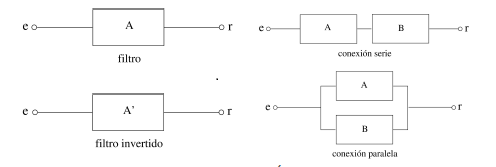
\includegraphics[scale=0.7]{figuras/conjuntos/ejercicio15/img1.png}
\end{figure}
Se considera ahora en el conjunto de todas las frecuencias y se identifica a cada filtro con el subconjunto
formado por aquellas fecuencias que éste deja pasar. Observar que con la identificación
recién establecida, se tienen las siguientes correspondencias:

 Filtro invertido $\Leftrightarrow$ Complemento , Conexión Serie $\Leftrightarrow$ Intersección , Conexión Paralela $\Leftrightarrow$ Unión
\begin{itemize}
	\item[i)] Diseñar circuitos para la construcción de los siguientes filtros  a partir de los filtros A,B y C.
	\begin{itemize}
		\item[(a)] $(A \cup B)^c$
				
				Gracias a las leyes de De Morgan, sabemos que:
				$$(A \cup B)^c = A^c \cap B^c$$ 
				Siguiendo las convenciones de los filtros, entonces podemos definir el siguiente filtro:
				\begin{figure}[H]
					\centering
		 			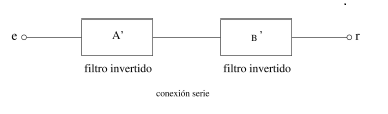
\includegraphics[scale=0.7]{figuras/conjuntos/ejercicio15/img2.png}
				\end{figure}
		
		\item[(b)] 	$(A \cap B)^c$
		
				Gracias a las leyes de De Morgan, sabemos que:
				$$(A \cap B)^c = A^c \cup B^c$$ 
				Siguiendo las convenciones de los filtros, entonces podemos definir el siguiente filtro:
				\begin{figure}[H]
					\centering
		 			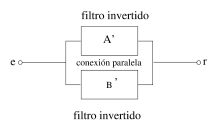
\includegraphics[scale=0.7]{figuras/conjuntos/ejercicio15/img3.png}
				\end{figure}
				
		\item[(c)] 	$A \cup (B \cap C)$
				\begin{figure}[H]
					\centering
		 			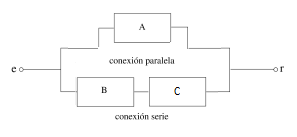
\includegraphics[scale=0.7]{figuras/conjuntos/ejercicio15/img4.png}
				\end{figure}		
		
		\item[(d)] 	$(A \cup B) \cap  (A \cup C)$
				\begin{figure}[H]
					\centering
		 			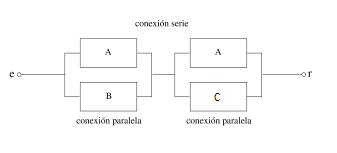
\includegraphics[scale=0.7]{figuras/conjuntos/ejercicio15/img5.png}
				\end{figure}
				Por las leyes distributivas sabemos que: $(A \cup B) \cap  (A \cup C) A \cup (B \cap C) $
				
				Por lo que también podríamos interpretar este como el circuito del inciso \textbf{(c)}
		\item[(e)] 	$(A \cap B) \cup  (A \cap C)$
			\begin{figure}[H]
					\centering
		 			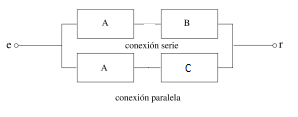
\includegraphics[scale=0.7]{figuras/conjuntos/ejercicio15/img6.png}
				\end{figure}
		\item[(f)] 	$A \vartriangle B$
		
		Acá debemos interpretar la diferencia simétrica en función de uniones, intersecciones y complementos. Entonces:
		$$A \vartriangle B = (A \cup B) - (A \cap B) = (A \cup B) \cap (A \cap B)^c = (A \cup B) \cap (A^c \cup B^c) $$
		Pasando esto a circuitos quedaría algo como :
		\begin{figure}[H]
					\centering
		 			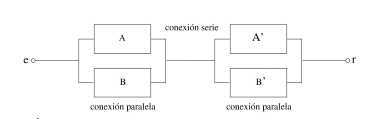
\includegraphics[scale=0.7]{figuras/conjuntos/ejercicio15/img7.png}
				\end{figure}
	\end{itemize}
	\item[ii)] Diseñar Circuitos para la construcción de los siguientes filtros a partir de los filtros A,B,C y D
	\begin{itemize}
		\item[(a)] $(D \vartriangle (A \cap B)) - C$
		\item[(b)] $((D \cap A) \vartriangle (D \cap B^c) )  \cup (A \cap B^c) \cap (C - D) ) $
		\item[(c)] $(A^c \cap B \cap C) \vartriangle (D^c \cap C)$
	\end{itemize}
\end{itemize} 
 
\end{ej}
---------------------------------------------------------------------------------------------------------------------------------------------
\begin{ej}
Sean $A= \{ 1,2,3 \}$, $B= \{ 1, 3, 5,7 \}$. Hallar $A \times A$ , $A \times B$, $(A \cap B) \times (A \cup B)$ 

\begin{itemize}
	\item $A \times A$: 
		$$A \times A = \{ 1,2,3 \} \times \{ 1,2,3 \} = \{ (1,1), (1,2), (1,3) , (2,1), (2,2), (2,3), (3,1) , (3,2), (3,3) \}$$
	\item $A \times B$: 	
		$$A \times B = \{ 1,2,3 \} \times \{ 1, 3, 5,7 \} = \{ (1,1), (1,3), (1,5) , (1,7), (2,1), (2,3), (2,5) , (2,7), (3,1), (3,3), (3,5) , (3,7) \}$$
	\item	$(A \cap B) \times (A \cup B)$
	$$(A \cap B) = (\{ 1,2,3 \} \cap  \{ 1, 3, 5,7 \}) = \{ 1, 3 \}$$
	$$(A \cup B) = (\{ 1,2,3 \} \cup  \{ 1, 3, 5,7 \}) = \{ 1, 2, 3, 5,7 \}$$
	Por lo que:
	$$(A \cap B) \times (A \cup B) = \{ 1, 3 \} \times \{ 1, 2, 3, 5,7 \} = \{ (1, 1), (1, 2), (1, 3), (1, 5), (1, 7), (3, 1), (3, 2), (3, 3), (3, 5), (3, 7)  \}$$
\end{itemize}

\end{ej}
---------------------------------------------------------------------------------------------------------------------------------------------
\begin{ej}
Sean A, B y C conjuntos. Probar que:
\begin{itemize}
	\item[i)] $(A \cup B) \times C = (A \times C) \cup (B \times C)$ 
	\item[ii)] $(A \cap B) \times C = (A \times C) \cap (B \times C)$
	\item[iii)] $(A - B) \times C = (A \times C) - (B \times C)$
	\item[iv)] $(A \vartriangle B) \times C = (A \times C) \vartriangle (B \times C)$
\end{itemize}
\end{ej}
---------------------------------------------------------------------------------------------------------------------------------------------
%------------------------------------------------------------------------------------------------------------------------------------%
%------------------------------------------------------------------------------------------------------------------------------------%
%------------------------------------------------------------------------------------------------------------------------------------%
\newpage


\subsection{Ejercicios Sobre relaciones }
\begin{ej}
Sean $A = \{ 1, 2, 3\}$ y  $B = \{ 1, 3, 5, 7\}$. Verificar si las siguientes son relaciones de $A$ en $B$ y en caso afirmativo graficarlas por medio de un diagrama con flechas de $A$ en $B$ y por medio de puntos en el producto cartesiano $A \times B$.
\begin{itemize}
	\item[i)] $\mathcal{R} = \{ (1,1), (1,3), (1,7), (3,1), (3,5)\}$
	\item[ii)] $\mathcal{R} = \{ (1,1), (1,3), (2,7), (3,2), (3,5)\}$
	\item[iii)] $\mathcal{R} = \{ (1,1), (1,3), (2,7), (3,3), (3,5)\}$
	\item[iv)] $\mathcal{R} = \{ (1,1), (1,3), (1,7), (3,1), (3,3), (3, 7)\}$
	\item[v)] $\mathcal{R} = \{ (1,1), (2,7), (3,7)\}$
	\item[vi)] $\mathcal{R} = \{ (1,3), (2,1), (3,7) \}$
\end{itemize}
\end{ej}

\begin{ej}
Sean $A = \{1,2,3\}$ y $B = \{1, 3, 5, 7\}$. Describir por extensión cada una de las relaciones siguientes de $A$ en $B$:
	\begin{itemize}
		\item[i)] $(a, b) \in \mathcal{R} \Leftrightarrow a \leq b$
		\item[ii)] $(a, b) \in \mathcal{R} \Leftrightarrow a > b$
		\item[iii)] $(a, b) \in \mathcal{R} \Leftrightarrow a \cdot b$
		\item[iv)] $(a, b) \in \mathcal{R} \Leftrightarrow a + b > 6$
	\end{itemize}	 
\end{ej}

\begin{ej}
Sea $A = \{ a, b, c, d, e, f, g, h\}$ para cada uno de los siguientes gráficos describir por extensión la relación en $A$ que representa y determinar si es reflexiva, simétrica, antisimetrica o transitiva.
\begin{figure}[H]
	\centering
	 \includegraphics[scale=0.7]{figuras/relaciones/img2.png}
\end{figure}
\end{ej}

\begin{ej}
Sea $A = \{ 1,2,3,4,5,6 \}$. Graficár la relación
$$\mathcal{R} = \{ (1,1), (1,3), (3,1), (3,3), (6,4), (4, 6), (4, 4), (6, 6) \}$$
\end{ej}

\begin{ej}
Sea $A = \{a,b,c,d,e,f \}$ y $\mathcal{R}$ la relación en A  representada por el gráfo:
\begin{figure}[H]
	\centering
	 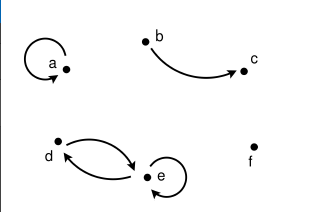
\includegraphics[scale=0.7]{figuras/relaciones/img3.png}
\end{figure}
Hallar la minima cantidad de pares que se deben agregar a $\mathcal{R}$ de manera que la nueva relación obtenida sea:
\begin{itemize}
	\item[(i)] Reflexiva
	\item[(ii)] Simetrica
	\item[(iii)] Transitiva
	\item[(iv)] Reflexiva y simetrica
	\item[(v)] Simetrica y transitiva
	\item[(vi)] De equivalencia
\end{itemize}
\end{ej}

\begin{ej}
En cada uno de los siguientes casos determinar si la relación $\mathcal{R}$ en $A$ es refexiva, simetrica, antisimetrica, transitiva de equivalencia o de orden.
	\begin{itemize}
		\item[(i)] $A =\{ 1,2,3,4,5\}$, $\mathcal{R} = \{ (1,1), (2,2), (3,3), (4, 4), (5, 5)\}$
		\item[(ii)] $A =\{ 1,2,3,4,5,6 \}$, $\mathcal{R} = \{ (1,1), (2,2), (3,3), (4, 4), (5, 5)\}$
		\item[(iii)] $A =\{ 1,2,3,4,5\}$, $\mathcal{R} = \{ (1,1), (2,2), (3,3), (4, 4), (5, 5), (1,2), (1,3), (2,5), (1,5)\}$
		\item[(iv)]$A = \mathbb{N}$, $\mathcal{R} = \{(a,b) \in \mathbb{N} \times \mathbb{N} :  a + b \, es \,  par \}$
		\item[(v)] $A = \mathbb{Z}$, $\mathcal{R} = \{(a,b) \in \mathbb{Z} \times \mathbb{Z} :  |a| \leq |b|  \}$
		\item[(vi)] $A = \mathbb{N}$, $\mathcal{R}$ definida por $a \mathcal{R} b \Leftrightarrow$ \textit{b} es multiplo de \textit{a}
		\item[(vii)] $A = \mathcal{P}(\mathbb{R})$, $\mathcal{R} $ definida por $\textbf{X} \mathcal{R} \textbf{Y}$ $\Leftrightarrow$ $\textbf{X} \cap \{1,2,3\} \subseteq \textbf{Y} \cap \{1,2,3\}$
	\end{itemize}
\end{ej}

\begin{ej}
 Sea $A$ unconjunto. describir todas las relaciones en A que son a la vez:
 \begin{itemize}
 		\item[i)] Simetricas y antisimetrica
 		\item[ii)] De equivalencia y de orden
 \end{itemize}
 ¿Puede una relación en A no ser no simetrica ni antisimetrica?
\end{ej}

\begin{ej}
Sea $A = \{ a,b,c,d,e,f \}$.  Dada la relación de equivalencia en $A$:
$$ \mathcal{R} = \{ (a,a), (b,b), (c,c), (d,d), (e,e), (f,f), (a,b), (b,a), (a, f), (f, a), (b, f), (f, b),(c, e),(e, c) \}$$
Hallar la clase $\overline{a}$ de $a$, la de $b$, la de $c$ y la de $d$, y la partición asociada a $\mathcal{R}.$
\end{ej}

\begin{ej}
Sea $A = \{ 1,2,3,4,5,6,7,8,9,10 \}$. Hallar y graficar la relaicón de equivalencia en $A$ asociada a la particion $\{ \{1,3\}, \{2,6,7\}, \{4,8,9,10\}, \{5\}   \}$. ¿Cuantas clases de equivalencia distintas tiene?. Hallar un representante para cada clase. 
\end{ej}

\begin{ej}
En el conjunto $\mathcal{Z}$ de números enteros, sea la relación de equivalencia dada por la paridad: dos números están relacionados si y solo si tienen la misma paridad (son ambos pares o ambos impares). ¿Cuántas clases de equivalencia distintas tiene? Hallar el representante mas simple posible para cada clase.
\end{ej}

\begin{ej}
En el conjunto $\mathbb{Z}$ de numeros enteros, sea la siguiente relación: dos números estan relacionados si terminan en el mismo digito. Verificar que es una relación de equivalencia. ¿Cuantas clases de equivalencia distintas tiene?. Hallar el representante mas simple posible para cada clase. 
\end{ej}

\begin{ej}
En el conjunto de todos los subconjuntos finitos de $\mathcal{N}$, sea la relación de equivalencia dada por el cardinal (es decir, la cantidad de elementos): dos subconjuntos están relacionados si y solo si tienen la misma cantidad de elementos. ¿Cuántas clases de equivalencia distintas tiene?. Hallar el representante más simple posible para cada clase.
\end{ej}
%------------------------------------------------------------------------------------------------------------------------------------%
%------------------------------------------------------------------------------------------------------------------------------------%
%------------------------------------------------------------------------------------------------------------------------------------%
\newpage
\section{Funciones}

\subsection{Ejercicios de Funciones}
\begin{ej}
Determinar que relaciones del ejercicio 18 son funciones de $A$ en $B$, y que relaciones del ejercicio 23 son funciones de $A$ en $A$
\end{ej}

\begin{ej}
Determinar si $\mathcal{R}$ es una función de $A$ en $B$ en los casos: 
\begin{itemize}
	\item[i)] $A = \{ 1,2,3,4,5 \}$ , $B = \{ a,b,c,d \}$, $\mathcal{R} = \{ (1,a), (2,a), (3,a), (4,b), (5,c), (3,d)\}$
	
	Acá vemos que el $3$ apunta a dos valores del codominio. Por lo que dicha relación no cumple con la definición de función
	\item[ii)] $A = \{ 1,2,3,4,5 \}$ , $B = \{ a,b,c,d \}$, $\mathcal{R} = \{ (1,a), (2,a), (3,d), (4,b)\}$
	
	Notemos que $5 \in A$ no se relaciona con ninguno de los elementos del codominio $B$. 
	
	Como la definición de función requiere de que todo elemento del dominio este relacionado con un elemento del codominio, entonces $\mathcal{R}$ no es función, ya que el 5 no se relaciona con ningún elemento del codominio.
	\item[iii)] $A = \mathbb{R}$, $B = \mathbb{N}$, $\mathcal{R} = \{ (a, b) \in \mathbb{R} \times \mathbb{N} / a = 2b - 3\}$
	
	El problema acá radica en que el dominio es más grande que el codominio, por lo que no se cumpliera que todo elemento del dominio se corresponda con un elemento del codominio.	
	
	\item[iv)] $A = \mathbb{Z}$, $B = \mathbb{Z}$, $\mathcal{R} = \{ (a, b) \in \mathbb{Z} \times \mathbb{Z} / a + b \, es \, divisible \, por \, 5\}$
	
	Acá necesitamos ver como demostrar que dado dos enteros siempre se puede tomar.
	
	Podemos ver que si se cumple que d es es divisible por 5, entonces $d - a = b$. 
	Por lo que, si $(a, d-a)$, entonces R es función.  
\end{itemize}
\end{ej}

\begin{ej}
Determinar si las siguientes funciones son inyectivas, sobreyectivas o biyectivas. Para las que sean biyectivas hallar la inversa y para las que no sean sobreyectivas hallar la imagen
\begin{itemize}
	\item[i)] $f: \mathbb{R} \rightarrow \mathbb{R}$, $f(x) = 12 x^2 - 5$
		
		En este caso, f es una cuadratica, por lo que no sera ni inyectiva ya que por ejemplo:
		$$f(-1) = f(1)$$
		Lo que nos descarta el hecho de que sea inyectiva. 
		
		Luego, como sabemos, para que sea sobreyectiva, debe cumplirse que $Im(f) = \mathbb{R}$ en este caso. Como vemos, la imagen es: $$Im(f) = \{ y : y \leq -5 \}$$	
		
		Por lo que no es sobreyectiva tampoco.
		
		Por ultimo, como no es ni inyectiva ni sobreyectiva no es biyectiva y no tiene inversa
	\item[ii)] $f: \mathbb{R}^2 \rightarrow \mathbb{R}$, $f(x, y) = x + y$
	
	Acá, en realidad tenemos una función de varias variables la cual de una función que depende de dos variables llegamos a un valor escalar. En particular
	\item[iii)] $f: \mathbb{R} \rightarrow \mathbb{R}^3$, $f(x) = (2 x, x^2, x - 7)$
	\item[iv)] 		
			$f: \mathbb{N} \rightarrow \mathbb{N}, f(n)=\left\{\begin{array}{cc}
				 \frac{n}{2} & \mbox{si n es par} \\
						n + 1 & \mbox{si n es impar}  \\
			 \end{array}\right.$	
			
	\item[v)] $f: \mathbb{Z} \times \mathbb{Z} \rightarrow \mathbb{Z}$, $f(a, b) = 3a - 2b$
	\item[vi)] 
			$f: \mathbb{N} \rightarrow \mathbb{N}, f(a)=\left\{\begin{array}{cc}
				 2a & \mbox{si a $>$ 0} \\
				1 - 2a & \mbox{si a $\leq$ 0}  \\
			 \end{array}\right. $	
			
\end{itemize}
\end{ej}

\begin{ej}
\begin{itemize}
	\item[i)] Dadas las funciones:
		\begin{displaymath}
			f: \mathbb{N} \rightarrow \mathbb{N}, f(n)=\left\{\begin{array}{cc}
				 \frac{n^2}{2} & \mbox{si n es divisible por 6} \\
						3n + 1 & \mbox{En los otros casos}  \\
			 \end{array}\right.	
		\end{displaymath}	
		$$g : \mathbb{N} \times \mathbb{N} \rightarrow \mathbb{N}, \, g(n, m) = (n(m + 1))$$
	
	Calcular $(f \circ g)(3,4) $, $(f \circ g)(2,5) $, $(f \circ g)(3,2) $ 				
	\item[ii)] Dadas las funciones:
			\begin{displaymath}
				f: \mathbb{R} \rightarrow \mathbb{R}, f(x)=\left\{\begin{array}{cc}
				 x^2 & \mbox{si x $\leq$ 7} \\
						2x - 1 & \mbox{si x > 7}  \\
			 \end{array}\right.	
		\end{displaymath}	
			$$g : \mathbb{N} \rightarrow \mathbb{R}  , \, g(n) = \sqrt{n}$$
	
	hallar todos los $n \in \mathbb{N}$ tales que $(f \circ g)(n) = 13$ y tales que $(f \circ g)(n) = 15$
\end{itemize}
\end{ej}

\begin{ej}
Hallar $(f \circ g)$ y $(g \circ f)$ (cuando se puede) en los casos:
\begin{itemize}
	\item[i)] $f : \mathbb{R} \rightarrow \mathbb{R}$, $f(x) = 2 x^2 - 18$ y $g : \mathbb{R} \rightarrow \mathbb{R}$, $g(x) =  x + 3$
	\item[ii)] 
	\begin{flushleft}		
	 	
				$f : \mathbb{N} \rightarrow \mathbb{N}, f(n)=\left\{\begin{array}{cc}
				 n - 2 & \mbox{si n es divisible por 4} \\
						n + 1 & \mbox{si n no es divisible por 4}  \\
			 \end{array}\right.$	
		y
			 $g: \mathbb{N} \rightarrow \mathbb{N}, g(n) = 4 n$
	\end{flushleft}	
	\item[iii)] $f : \mathbb{R} \rightarrow \mathbb{R} \times \mathbb{R}$, $f(x) = (x + 5, 3 x)$ y $g : \mathbb{N} \rightarrow \mathbb{R}$, $g(n) = \sqrt{n}$
	
\end{itemize}

\end{ej}

\begin{ej}
Hallar dos funciones $f: \mathbb{N} \rightarrow \mathbb{N}$ y $g: \mathbb{N} \rightarrow \mathbb{N}$ tales que $f \circ g = id_{\mathbb{N}}$ y $g \circ f \cancel{=} id_{\mathbb{N}}$, donde $id_{\mathbb{N}}: \mathbb{N} \rightarrow \mathbb{N}$
\end{ej}

\begin{ej}
Sean $A$, $B$ y $C$ conjuntos. Probar que si $f: B \rightarrow C$ y $g: A \rightarrow B$ son funciones entonces valen
\begin{itemize}
	\item[i)] Si $f \circ g$ es inyectiva entonces $g$ es intectiva.
	\item[ii)] Si $f \circ g$ es sobreyectva entonces $f$ es sobreyectiva.
	\item[iii)] Si $f \circ g$ son inyectivas entonces $f \circ g$ es inyectiva. 
	\item[iv)] Si $f \circ g$ son sobreyectivas entonces $f \circ g$ es sobreyectiva.
	\item[v)] Si $f$ y $g$ son biyectivas entonces $f \circ g$ es biyectiva.
\end{itemize}
\end{ej}
%------------------------------------------------------------------------------------------------------------------------------------%
%------------------------------------------------------------------------------------------------------------------------------------%
%------------------------------------------------------------------------------------------------------------------------------------%
\newpage
\section{Números Naturales}

\subsection{Ejercicios Sobre Numeros Naturales}
\begin{ej}
\begin{itemize}
\item[i)] Reescribir cada una de las siguientes sumas usando el símbolo de sumatoria
\begin{itemize}
\item[(a)] $1 + 2 + 3 + 4 + \cdots + 100$
La solución a esta sucesion es basicamente la formula de gauss:
\[\sum_{i=1}^{10} = \frac{2^{32+1}}{2-1}\]
(No hace falta hacer una demostración)
\item[(b)] $1 + 2 + 4 + 8 + 16 + \cdots + 1024$
Esta sucesion puede verse facilmente que es $2^i$ donde $i$ va desde 0 hasta 32:
\[\sum_{i=0}^{32} 2^i = \frac{2^{11} - 1}{2 - 1} = 2047\]
\item[(c)] $1 + (-4) + 9 + (-16) + 25 + \cdots + (-144)$
\[\sum_{i=0}^{12} {-1}^{i+1} i^2 \]
\item[(d)] $1 + 9 + 25 + 49 + \cdots + 441$
\[\sum_{i=0}^{10} (2i +1)^2 \]
\item(e)] $1 + 3 + 5 + \cdots + (2n + 1)$
\[\sum_{i=0}^{n} (2i +1)^2 \]
\item[(f)] $n + 2n + 3n + \cdots + n^2$
\[\sum_{i=1}^{n} i  n \]
\end{itemize}

\item[ii)] Reescribir cada una de los siguientes productos usando el símbolo de productoria y/o de
factorial
\begin{itemize}
\item[(a)] $5 \cdots 6 \cdots 99 \cdot 100$
\[\prod_{i=5}^{100} i = \cfrac{\prod_{i=1}^{100} i}{\prod_{i=1}^{4} i} = \frac{100!}{4!}\]
\item[(b)] $1 \cdot 2 \cdot 4 \cdot 8 \cdot 16 \cdots 1024$
\[\prod_{i=0}^{10} 2^i \]
\item[(c)] $n \cdot 2n \cdot 3n \cdots n^2$
\[\prod_{i=1}^{n} i n = \prod_{i=1}^{n} i \prod_{i=1}^{n}  n = n! * n^n\]
\end{itemize}
\end{itemize}
\end{ej}

\begin{ej}
Calcular
\begin{itemize}
\item[i)] $\sum_{i=1}^{n} 4i + 1$

\solucion

\[\sum_{i=1}^{n} 4i + 1 = 4 \sum_{i=1}^{n} i + \sum_{i=1}^{n} 1 = 4 \left( \frac{n(n+1)}{2}\right) + n = 2n(n+1) + n = \resultado{n(2n+2)}\]
\item[ii)] $\sum_{i=6}^{n} 2(i -5)$

\solucion

\[\sum_{i=6}^{n} 2(i -5) = \sum_{i=6}^{n} (2i -10) = \sum_{i=1}^{n} (2i -10) - \sum_{i=1}^{6} (2i - 10) = 2 \overbrace{\left(\sum_{i=1}^{n} i\right)}^{Gauss} - \left(\sum_{i=1}^{n} 10 \right) - 2 \overbrace{\left(\sum_{i=1}^{6} i \right)}^{Gauss} + \left(\sum_{i=1}^{6} 10\right)=\]
\[ 2 \frac{n(n+1)}{2} - 10 n - 2 \frac{6(7)}{2} + 6 (10) = n(n+1) - 10 n - 42 + 60 = \resultado{n((n+1) - 10) + 18}\]
\end{itemize}
\end{ej}

\begin{ej}
Probar $\forall$ $n \in \mathbb{N}$ 
\begin{itemize}
\item[i)] $\sum_{i=1}^{n} i^2 = \frac{n(n+1)(2n+1)}{6}$

\solucion
\\\\
\ttfamily
Pobaremos esto por inducción:

Nuestra proposición es  $\sum_{i=1}^{n} i^2 = \frac{n(n+1)(2n+1)}{6}$

Debemos probar: (1) caso base y (2) el paso inductivo.

\begin{enumerate}
\item \textbf{Caso Base}: ¿$p(1)$ es verdadero?

\[\sii \sum_{i=1}^{1} i^2 = \frac{1(1+1)(2 (1)+1)}{6} \sii 1^2 = \frac{2 + 3}{6} \sii 1=1\]
Lo cual es cierto. $\therefore$ el caso base es verdadero.

\item \textbf{Paso Inductivo}: Supongo que $p(h)$ es verdadero y quiero ver si $p(h) \implica p(h+1)$. 

Encaremos esto:
\[\sum_{i=1}^{n+1} i^2 = \sum_{i=1}^{n} i^2 + (n+1)^2 \overbrace{=}^{H.I.} \frac{n(n+1)(2n+1)}{6} + (n+1)^2 = \frac{n(n+1)(2n+1) + 6(n+1)^2}{6}\]
\[= \frac{(n+1)(n(2n+1) + 6(n+1))}{6} = \frac{(n+1)(2n^2 + n + 6n+6))}{6} = \resultado{\frac{(n+1)(2n^2 + 7n + 6))}{6}}\]

Lo cual es cierto, ya que, si $p(h) = \frac{n(n+1)(2n+1)}{6}$ 
\[\implica p(h+1) = \frac{(n+1)(n+2)(2(n+1)+1)}{6} = \frac{(n+1)(n+2)(2n +3)}{6} = \resultado{\frac{(n+1)(2n^2 + 7n + 6)}{6}}\]

$\therefore$ Tenemos que $p(h) \implica p(h+1)$ es verdadero, entonces $p(n)$ es verdadero $\forall$ $n \in \mathbb{N}$
\end{enumerate}

\newpage
\item[ii)] $\sum_{i=1}^{n} i^3 = \frac{n^2(n+1)^2}{4}$

\solucion
\\\\
Debemos probarlo por inducción.

$p(h): \sum_{i=1}^{h} i^3 = \frac{h^2(h+1)^2}{4}$
\begin{enumerate}

\item \textbf{Case Base}: ¿$p(1)$ es verdadero?

\[\sum_{i=1}^{1} i^3 = \frac{1^2(1+1)^2}{4} \sii 1^3 = \frac{4}{4} \sii 1=1\]
Lo cual es cierto. $\therefore$ el caso base es verdadero.

\item \textbf{Paso Inductivo}: Supongo que $p(h)$ es verdadero y quiero ver si $p(h) \implica p(h+1)$. 
\[\sum_{i=1}^{h+1} i^3 = \sum_{i=1}^{h} i^3 + (h+1)^3 \overline{=}^{H.I} \frac{h^2(h+1)^2}{4} + \frac{4(h+1)^3}{4} = \frac{h^2(h+1)^2 + 4(h+1)^3}{4} = \]
\[ = \frac{(h+1)^2(h^2 + 4(h+1))}{4} = \frac{(h+1)^2(h^2 + 4h + 4))}{4} = \resultado{\frac{(h+1)^2(h+2)^2)}{4}}\] 

Lo cual es cierto, ya que, si $p(h) = \frac{h^2(h+1)^2}{4}$. Entonces:
\[\resultado{p(h+1) = \frac{(h+1)^2 (h+2)^2}{4}}\] 

$\therefore$ Tenemos que $p(h) \implica p(h+1)$ es verdadero, entonces $p(n)$ es verdadero $\forall$ $n \in \mathbb{N}$
\end{enumerate}




\end{itemize}
\end{ej}


\newpage
\section{Combinatoria}

\subsection{Ejercicios Sobre Combinatoria }

\caja{1}{0.9}{
\begin{ej}
Dado el conjunto referencial $V = \lbrace n \in \mathbb{N} : n$ es multiplo de $15 \rbrace$, determinar el cardinal del complemeto del subconjunto $A$ de $V$ definido por:
$A = \lbrace n \in V : n \mayig 132 \rbrace$
\end{ej}
}

\vspace{0.5cm}

\solucion

\vspace{0.5cm}

Los múltiplos de un número son todos los posibles resultados de multiplicar ese número por todos y cada uno de los números naturales.

Por otro lado, nosotros queremos saber la cantidad de elmentos que hay en $A^c$ es decir, como el conjunto $A$ son todos los multiplos de 15 mayores a 132, entonces el 
complemento son todos los multiplos de 15 menores a 132. Veamos:
\[15 \cdot 1 = 15, \hspace{0.2cm} 15 \cdot 2 = 30 , \hspace{0.2cm} 15 \cdot 3 = 45 , \hspace{0.2cm} 15 \cdot 4 = 60 , \hspace{0.2cm} 15 \cdot 5 = 75 , \hspace{0.2cm}
15 \cdot 6 = 95 , \hspace{0.2cm} 15 \cdot 7 = 105 , \hspace{0.2cm} 15 \cdot 8 = 120 , \hspace{0.2cm}\]
Luego, $A^c$ es el conjunto dado por:
\[A^c = \lbrace 15,30,45,60,75,95,105,120 \rbrace \]
El cual tiene $8$ elementos.

\rojo{$\therefore \# (A^c) = 8$}

\vspace{0.5cm}

\caja{1}{0.9}{
\begin{ej}

¿Cuántos números naturales hay menores o iguales que $1000$ que no son, ni multiplos de $3$, ni multiplos de $5$?
\end{ej}
}

\vspace{0.5cm}

\solucion

\vspace{0.5cm}

Este ejercicio es medio al pedo. Basicamente tenes que tomar el conjunto de los elementos del 1 al 1000, tal que todos los elementos son naturales. Luego, tengo que sacarle los conjuntos de los multiplos de 3 y los multiplos de 5 y tomar el cardinal de los elementos que quedan. 

Multiplos de 5:
\[5, 10, 15, 20, 25, 30, 35, 40, 45, 50, 55, 60, 65, 75, 80, 85, 90, 95, 100\]
Estos son los primeros 19 valores que son multiplos de 5 hasta llegar a 100, luego como esta cantidad se repite de 100 a 200, tenemos $19 \cdot 10 = 190$. Por lo tanto, tenemos 190 elementos dentro de los multiplos de 5 menores o iguales a 1000. 

Multiplos de 3:
\[3, 6, 9, 12, 15, 18, 21, 24, 27, 30, 33, 36, 39, 42, 45, 48, 51, 54, 57, 60, 63, 66, 69, 72, 75, 78, 81, 84, 87, 90, 93, 96, 99\]
Luego, tenemos 33 valores para los naturales menores iguales a 100. Por otro lado, podemos notar que cada 5 valores tenemos 1 multiplo que es tanto de 3 como de 5, por lo que deberiamos sacar esta cantidad del conjunto de numeros multiplos de 3. Es decir, el conjunto de los multiplos de 3 y de los multiplos de 5 no es disjunto. 

Tenemos $33 \cdot 10 = 330$ elementos dentro del conjunto de multiplos de 3 menores a 1000. Por otro lado, tenemos $190/5 = 45$ son 45 elementos que son tanto multiplo de 3 como de 5. Por lo tanto, la unión entre los conjuntos de multiplos de 3 y de 5 es: $330 + 190 - 45 = 475$

Luego, la cantidad de elementos dentro del conjunto de numeros menores iguales a 1000 que son multiplos de 3 y de 5 son $475$ elementos, como queremos el complemento entonces : $1000 - 475 = 525$ elementos

\vspace{0.5cm}
  
\caja{1}{0.9}{
\begin{ej}

Dados los subconjuntos finitos $A;B;C$ de un conjunto referencial $V$ , calcular 
$\#(A \union B \union C)$ en términos de los cardinales de $A$, $B$, $C$ y sus intersecciones.
\end{ej}
}

\vspace{0.5cm}

\solucion

\vspace{0.5cm} 
 
 Suponiendo que no son disjuntos. Como : $\#(A \union B) = \#(A) + \#(B) - \#(A \interseccion B)$
 
 Podemos suponer que va a pasar lo mismo con:$\#(A \union C) = \#(A) + \#(C) - \#(A \interseccion C)$
 
 Y con:
 $\#(B \union C) = \#(B) + \#(C) - \#(B \interseccion C)$
 
 Por lo tanto: 
 $$\#(A \union B \union C) =\#(A) + \#(B) + \#(C) - \#(A \interseccion B) - \#(A \interseccion C) - \#(B \interseccion C)$$
 Que es lo mismo que:
$$\rojo{\#(A \union B \union C) = \#(A) + \#(B) + \#(C) - ( \#(A \interseccion B) + \#(A \interseccion C) + \#(B \interseccion C))}$$
 
\vspace{0.5cm}
  
\caja{1}{0.9}{
\begin{ej}

\begin{itemize}

\item[i) ] Una compañia tiene 420 empleados de los cuales 60 obtuvieron un aumento y un ascenso,
240 obtuvieron solo un aumento y 115 obtuvieron solo un ascenso. ¿Cuántos empleados no
obtuvieron ni aumento ni ascenso?

\item[ii) ] En el listado de inscripciones de un grupo de 150 estudiantes, donde hay 83 inscripciones en
Análisis y 67 en Álgebra. Además se sabe que 45 de los estudiantes se anotaron en ambas
materias. ¿Cuántos de los estudiantes no están inscriptos en ningún curso?

\item[iii) ] En un instituto de idiomas donde hay 110 alumnos, las clases de inglés tienen 63 inscriptos,
las de alemán 30 y las de francés 50. Se sabe que 7 alumnos estudian los tres idiomas, 30
solo estudian inglés, 13 solo estudian alemán y 25 solo estudian francés. ¿Cuántos alumnos
estudian exactamente dos idiomas? ¿Cuántos inglés y alemán pero no francés? ¿Cuántos no
estudian ninguno de esos idiomas?
\end{itemize}
\end{ej}
}

\vspace{0.5cm}

\solucion

\begin{itemize}
\item[i) ]
Luego de leerlo varias veces, pude entender que me pide los que no les dieron ni aumento, ni ascenso. Como a los que le dieron ambas cosas no estan dentro de los que les dieron solo ascenso o de los que les dieron solo aumento, se cumple que, si $E =420$ es el total de empleados del conjunto referencial, y $A$ y $B$ son los conjuntos de aumento y ascenso
$$\# E - \#(A \cup B) =\# E - ( \# A + \# B - \#(A \cap B))= \# E - \# A - \# B + \#(A \cap B) = 420 - 240 -115 + 60 = \rojo{125}$$ 

\item[ii) ]
Al igual que antes, tenemos la unión de dos conjuntos:
$$\# E - \#(An \cup Al) =\# E - ( \# An + \# Al - \#(An \cap Al))= \# E - \# An - \# Al + \#(An \cap Al) = 150 - 83 - 67 + 45 = \rojo{45}$$ 

\item[iii) ]
Para este ejercicio tenemos algo mas molesto. Tenemos la siguiente situacion:

\begin{minipage}[b]{0.5\linewidth}
\begin{itemize}
	\item $\#(A) = 30 = 13 + x + 7 + z \hspace{0.2cm} \sii \hspace{0.2cm} 10 = x + z \hspace{0.2cm} (1)$
	\item $\#(I) = 63 = 30 + y + z + 7 \hspace{0.2cm} \sii \hspace{0.2cm} 26 = x + y \hspace{0.2cm} (2)$
	\item $\#(F) = 50 = 25 + 7 + y + z \hspace{0.2cm} \sii \hspace{0.2cm} 18 = y + z \hspace{0.2cm} (3)$
	\item $\#(A \interseccion I \interseccion F) = 7$
Nesesitamos calcular quienes son $x$, $y$, $z$ para luego responder las insoportables pregutas. Esto lo acemos como cualquier sistema de ecuaciones:

De (1):
\[ z = 10 - x \]
Meto en (3):
\[ 18 = y + 10 - x \hspace{0.2cm} \sii \hspace{0.2cm} 8 + x = y \]
\end{itemize}
\end{minipage}
\begin{minipage}[b]{0.5\linewidth}
		\centering
		%%%%%%%%%%%%%%%%%%%%%%%%%%%%%%%%%%%%%%%%%%%%%%%%%%%%%%%%%%%
		% 			UNION DE TRES CONJUNTOS 
		%%%%%%%%%%%%%%%%%%%%%%%%%%%%%%%%%%%%%%%%%%%%%%%%%%%%%%%%%%%
 \begin{tikzpicture}
   	\draw (-2, 2.5) rectangle (3, -2.5);
   	\draw (-2.4,2.6) node {$V$};   
   
    %Es importante que el orden en el que se van mostrando los objetos
    % Se Respete
    
	%El cirulo C se pinta de azul   
   	\fill[color=blue!20!white] (0.5,1) circle (1); 
	%Los cirulos A y B se pintan de Blanco   
   	\fill[color=blue!20!white] (0,0) circle (1);
   	\fill[color=blue!20!white] (1,0) circle (1); 

	%Interseccion AC superior izquierdo
	\begin{scope}
 		\clip (0.5,1) circle (1);
  		\clip (0,0) circle (1);
  		\fill[color=blue!20!white] (0,0) circle (1);
  		%\fill[color=white] (1,0) circle (1);
 	 \end{scope}
  	
  	%Interseccion BC superior derecho
  	\begin{scope}
  		\clip (0.5,1) circle (1);
  		\clip (1,0) circle (1);
  		\fill[color=blue!20!white] (1,0) circle (1);
  		%\fill[color=white] (0,0) circle (1);
  	\end{scope}
  	
  	%Interseccion AB Inferior
  	\begin{scope}
  		\clip (0,0) circle (1);
  		\clip (1,0) circle (1);
  		\fill[color=blue!20!white] (1,0) circle (1);
  		\fill[color=white] (0.5,1) circle (1);
  	\end{scope} 

	% Interseccion entre los tres conjuntos (centro)
	\begin{scope}
 		\clip (1,0) circle (1);
 		\clip (0.5,1) circle (1);
 		\clip (0,0) circle (1);
 		\fill[color=blue!20!white] (-2, 2.5) rectangle (3, -2.5); 
 	\end{scope}	
	

   
	%Posicion circulo A	   
   	\draw (0, 0) circle (1);
   	\draw (-0.7,-1.2) node {$A$};
   
   	%Posicion circulo B
   	\draw ( 1, 0) circle (1);
   	\draw (1.7,-1.2) node {$I$};
  
   	%Posicion circulo C
   	\draw (0.5,1)circle (1);
   	\draw (1.7,1.5) node {$F$};
   	
   	% Nodos
   	\draw (0.5,1.5) node {$25$};
   	\draw (0.5,0.5) node {$7$};
   	\draw (1.1,0.5) node {$z$};
   	\draw (-0.1,0.5) node {$y$};
   	\draw (0.5,-0.3) node {$x$};
   	\draw (-0.5,-0.4) node {$13$};
   	\draw (1.3,-0.4) node {$30$};
 \end{tikzpicture}

	Unión de los Tres conjuntos
\end{minipage}

\end{itemize}
Luego, meto este ultimo resultado en (2):
\[26 = x + 8 + x \hspace{0.2cm} \sii \hspace{0.2cm} 18 = 2x \hspace{0.2cm} \sii \hspace{0.2cm} \rojo{x = 9}\]
Meto este resultado en las ecuaciones (1) y (2) para calcular $y$ y $z$:
\[10 = x + z \hspace{0.2cm} \sii \hspace{0.2cm} \rojo{ z =  1 } \]
\[26 = x + y \hspace{0.2cm} \sii \hspace{0.2cm} \rojo{ y = 17 } \]

\textbf{¿Cuántos alumnos estudian exactamente dos idiomas?}

Esto es: $x + y +z = 9 + 17 + 1 = \rojo{27}$ 

\textbf{¿Cuántos inglés y alemán pero no francés? }

Esto es: $13 + x + 30 = 13 + 9 + 30 = \rojo{52}$

\textbf{¿Cuántos no estudian ninguno de esos idiomas?}

Esto es: 

$x + y + z + 13 + 30 + 25 + 9 + 17 + 7 = 92$

Luego tenemos $\#V = 110$ por lo que tenemos:

$$ 110 - 92 = \rojo{18} $$

\vspace{0.5cm}  
 
 
\caja{1}{0.9}{
\begin{ej}

Si hay 3 rutas distintas para ir de Buenos Aires a Rosario, 4 rutas distintas para ir de Rosario a
Santa Fe, y 2 para ir de Santa Fe a Reconquista ¿cuántos formas distintas hay para ir de Buenos
Aires a Reconquista pasando por las dos ciudades intermedias?
\end{ej}
}

\vspace{0.5cm}

\solucion 
 
\vspace{0.5cm}

\[4 \cdot 3 \cdot 2 = 24\] 

\vspace{0.5cm}

\caja{1}{0.9}{
\begin{ej}
	
	\begin{itemize}
		\item[•]
		\item[i)  ] ¿Cuántos números de exactamente 4 cifras (no pueden empezar con 0) hay que no contienen al dígito 5?
						
		\item[ii) ] ¿Cuántos números de exactamente 4 cifras hay que contienen al dígito 7?
	\end{itemize}
\end{ej}
}

\vspace{0.5cm}

\solucion 
\begin{itemize}
	\item[i) ]
			Pensemos, un poco. Podemos crearnos dos funciones inyectivas $\varphi$ y $\phi$ tal que ambas son inyectivas. Definimos estas como:
		
		\[\varphi : 4 \rightarrow 8 \hspace{0.5cm} \land \hspace{0.5cm} \varphi : 1 \rightarrow 3 \]
		Es decir, la función que manda cada elemento de los 8 elementos a uno de cuatro y otra que distribuye 1 elementro entre tres lugares (plantemos la inversa)
		
		Luego, la solución al problema sera: $\#(\mathcal{N}) = \#(\varphi) \cdot \#(\phi)$  
		
		El cardinal de una función inyectiva $f: A_m \rightarrow B_n$ esta dado por $\frac{n!}{(n-m)!}$. 
		\[\therefore \#(\mathcal{N}) = \#(\varphi) \cdot \#(\phi)  = \frac{8!}{(8-4)!} \cdot \frac{3!}{(3-1)!} = \frac{8\cdot7\cdot6\cdot5\cdot \cancel{4!}}{\cancel{4!}} \cdot \frac{3 \cdot \cancel{2!}}{\cancel{2!}} = \rojo{5040}\]	

	\item[ii) ]
			
\end{itemize}
 
\vspace{0.5cm}
 
 
 \subsection{Ejercicios de las clases}
%%%%%%%%%%%%%%%%%% 
\caja{1}{1}{
\textbf{Clase del 2-10-2020}
Definiciones de Cantidad de funciones inyectivas y de funciones biyectivas. Ver resumen. 

\begin{ej}

Sea $1 \menig k \menig n$. Probar que $k \comb{n}{k} = n \comb{n-1}{k-1}$

Hagamos la cuenta:
\[k \comb{n}{k} =  k \frac{n !}{k! (n-k)!} = \frac{n !}{(k-1)! (n-k)!}\]

\[n \comb{n-1}{k-1} = n \frac{(n-1) !}{(k-1)! (n-k)!} = \frac{n !}{(k-1)! (n-k)!}\]

\end{ej}

\begin{ej}

Sean $k, m \mayig 0$ talque $k+m \menig n$. Probar que
\[\comb{n}{k} \comb{n-k}{m} = \comb{n}{m} \comb{n-m}{k}\]

\textbf{Lado izquierdo de la igualdad:}

Esto es: Tengo $n$ personas saco $k$ personas  y de la cantidad de gente que queda $(n-k)$ elijo m personas

\textbf{Lado derecho de la igualdad}

Elegimos de las $n$ a m personas que se van y las $n-m$ pestonas que quedaron se van $k$
\end{ej}

\begin{ej}
Sea $n \mayig 3$ donde $[n] = \lbrace 1,2,3,...,n \rbrace$ ¿Cuantas relaciones de Equivalencia se pueden definir en [n] de modo tal que la clase de 1 tenga n-2 elementos?

\[\comb{n-1}{2} + \comb{n-1}{2}\]
\end{ej}

\begin{ej}

¿Cuantas relaciones de equivalencia hay en $[n] = \lbrace 1,2,3,...,n \rbrace$ con exactamente 2 clases de equivalencia? 

\[\frac{2^{n} - 2}{2} = 2^{n-1} - 1\]

\end{ej}
} 
 

 
 
 
 
\section{Referencias}
\href{https://tex.stackexchange.com/}{stackexchange}
%%%%%%%%%%%%%%%%%%%%%%%
%	TextColor
%%%%%%%%%%%%%%%%%%%%%%%
%\textcolor{B}{}

%\begin{table}[H]
%	\begin{center}
%		\begin{tabular}{|c|c|c|c|c|c|}
%			\hline
%				 0 & 0  &  1  &  0  &   0   &   1   \\ 
% 			\hline
%		\end{tabular}
%		\caption{}
%		\label{tabla:sencilla}
%	\end{center}
%\end{table}	

%%%%%%%%%%%%%%
%    CAJAS   %
%%%%%%%%%%%%%%

%\begin{center}
%\fbox{\begin{minipage}[b][1.5\height]%
%[t]{0.7\textwidth} texto incluido
%dentro de una caja construida con
%el entorno minipage. Nótese como
%por defecto  es 0pt dentro
%de las minipage
%\end{minipage}}
%\end{center}


%\begin{array}{ccc}
% \hat{i} & \hat{j} & \hat{k} \\
%		a_1 & a_2 &  a_3 \\
%		b_1 & b_2 &  b_3
% \end{array}

%%%%%%%%%%%%%%%%%%%%%%%
%					Minifiguras
%%%%%%%%%%%%%%%%%%%%%%%
%\begin{figure}[H]
%	\begin{minipage}[b]{0.6\linewidth}
%		\centering
%		 \includegraphics[scale=0.7]{figuras/clase1/img2.png}
%	\end{minipage}	 	
%	\begin{minipage}[b]{0.4\linewidth}	
%	\end{minipage}
%\end{figure}

\end{document}
